\documentclass[a4paper,11pt]{article}
\pdfoutput=1 % if your are submitting a pdflatex (i.e. if you have
             % images in pdf, png or jpg format)

\usepackage{jinstpub} % for details on the use of the package, please
                     % see the JINST-author-manual

\usepackage[utf8]{inputenc}

\usepackage{lineno}
\usepackage{color}
\newcommand{\todo}[1]{\textcolor{red}{{#1}}}
\usepackage[outdir=./]{epstopdf}

\linenumbers

\title{\boldmath Commissioning of the highly granular SiW-ECAL technological prototype}

% e-mail addresses: only for the forresponding author
\emailAdd{irles@lal.in2p3.fr}
%\collaboration[]{on behalf of the CALICE collaboration}


\abstract{
  High precision physics at future colliders as the International Linear Collider (ILC) require unprecedented high precision in the determination
  of the final state of the particles produced in the collisions
  The needed precision will be achieved thanks to the Particle Flow algorithms (PF) which require compact, highly granular and hermetic calorimeters systems.
  The Silicon-Tungsten Electromagnetic Calorimeter (SiW-ECAL) technological prototype
  design and R\&D is oriented at the baseline design of the ECAL of the International Large Detector (ILD) for the ILC.
  In this article we present the commissioning and the performance of the prototype in our beam test carried at DESY in June 2017.
}


\keywords{Calorimeter methods, calorimeters, Si and pad detectors}


\begin{document}
\maketitle
\flushbottom


\section{Introduction}

Future accelerator based particle physics experiments
require very precise and detailed reconstruction of the final states produced
in the beam collisions. A particular example is the next generation of $e^{+}e^{-}$
linear colliders such the ILC\cite{Behnke:2013xla,Baer:2013cma,Adolphsen:2013jya,Adolphsen:2013kya,Behnke:2013lya}.
This project will provide collisions of polarized beams with center-of-mass energies ($c.m.e$) of 250 GeV - 1 TeV.
These collisions will be studied by two multipurpose detectors:
the International Large Detector (ILD) and the Silicon Detector (SiD)\cite{Behnke:2013lya}.
To meet the precision levels required by the ILC %or CLIC
physics goals,
new techniques relying on single particle separation to make possible the choice of the best information available
in the full detector to measure the energy of the final state objects have been developed.
These techniques are called Particle Flow (PF) techniques \cite{Brient:2002gh,Morgunov:2004ed,Sefkow:2015hna}
and allow to reduce the impact of the poor resolution of the calorimeter systems (compared with trackers) in the overall reconstruction.
The PF algorithms impose some special requirements in the design of the detectors.
For example, it requires highly granular, compact
and hermetic calorimeters.

The CALICE collaboration is driving most of the efforts on R\&D of highly granular calorimeters \cite{Sefkow:2015hna} 
for future linear colliders by investigating and building prototypes for several
calorimeter concepts. One of these calorimeters 
is the silicon-tungsten electromagnetic calorimeter, SiW-ECAL.
The SiW-ECAL is the baseline choice for the ILD electromagnetic calorimeter.
It consists of a detector (in the barrel region) of 24 $X_{0}$ of thickness which corresponds to $\sim 1~\lambda_{I}$ (interaction length).
It has silicon (Si) as active material and tungsten (W) as absorber material.
The combination of Si and W choices  makes possible the design and construction
of a very compact calorimeter with highly granular and compact active layers.
It will be built an alveolar structure of carbon fiber into which modules made of tungsten
plates and the active sensors will be inserted. The very-front-end (VFE) electronics will be
embedded in the detector units. The silicon sensors will be segmented
in squared cells (or channels) of 5x5 mm: a total of $\sim 100$ million readout channels will constitute the ECAL for ILD.
The desired signal dynamic range in each channel goes from 0.5 MIP to 3000 MIPs, where the MIP acronym stands 
for the energy deposited by a minimum-inonizing-particle.
To reduce overall power consumption, the SiW-ECAL will exploit the special bunch structure
foreseen for the ILC: the $e^{+}e^{-}$ bunches trains will arrive in spills
of $\sim$ 1-2 ms width separated by $\sim$ 200 ms. The data acquisition will be gated during these short windows and during the idle time the bias currents of the electronics will be shut down.
This technique is usually denominated power pulsing. In addition to this, to cope with the large amount of channels,
the calorimeters should work in self-trigger mode (each channel featuring an internal trigger decision chain) and zero suppression mode. 

\section{The SiW-ECAL technological prototype}

The first SiW-ECAL prototype was the so called SiW-ECAL physics prototype.
It was successfully tested at DESY, FNAL and CERN running in front of another prototype from the CALICE
collaboration, the analogue hadronic calorimeter AHCAL, delivering the proof of concept of the technollogy
and the PF calorimetry.
For the physics prototype, the VFE was placed outside the active area with no particular constraints in power consumption.
It consisted of 30 layers of Si as active material alternated with tungsten plates as absorber material.
The active layers were made of a matrix of 3x3 Si wafers of 500 $\mu$m thickness. Each of these wafers was segmented in matrices of
6x6 squared channels of 1x1 $cm^{2}$, allowing for a potential density of 1500 channels/dm$^{3}$ assuming
the ILD baseline design constraints on the material repartition and compactness.
The prototype was divided in 3 modules of 10 layers with different W depth per layer in each of these modules
(0.4, 1.6 and 2.4 $X_{0}$) making a total of 24 $X_{0}$.
That very first prototype offered a signal over noise on the measured charge of 7.5 for MIP like 
particles. More results proving the good performance of the technology and the PF can be found in
references~\cite{Adloff:2011ha,Anduze:2008hq,Adloff:2008aa,Adloff:2010xj,CALICE:2011aa,Bilki:2014uep}.

The current prototype is called the SiW-ECAL technological prototype. It addresses the main technological challenges: compactness,
power consumption reduction through power pulsing and VFE inside the detector close to real ILD conditions.
It will also provide data to deeply study the PF and provide input to tune simulation programs as for example
GEANT4\cite{Agostinelli:2002hh,Allison:2006ve,Allison:2016lfl} which is widely used
in particle physics to simulate the passage of particles through matter. In this section we described in detail
the main features and characteristics of the technological prototype.

\subsection{Silicon sensors}
\label{sec:wafers}

The sensors consist of high resistivity (bigger than 5000 $\Omega\cdot$cm)
%floating zone
silicon wafers with a thickness of 320$\mu$m.
The size of the wafers is $9\times9$ cm$^{2}$ and they are each subdivided in an array of 256 PIN diodes of $5\times5$ mm$^{2}$.
A MIP traversing the PIN parallel to its normal will create $\sim$ 80 $h^{+}e^{-}$ pairs per $\mu$m which corresponds to 4.1 fC
for particles incident perpendicularly to its surface.

The original design of the silicon wafers included an edge termination made of floating guard-rings.
It was observed in beam tests \cite{Cornat:2015eoa,Cornat:2009zz} that the capacitive coupling between such floating guard-rings 
and the channels at the edge created not negligible rates off fake
events in tests with high energy beams (pions and electrons with energies larger than 20-40 GeV)
An R\&D program together with Hamamatsu Photonics (HPK Japan) was conducted to study the guard-rings design 
as well as the internal crosstalk. It was concluded that using wafers without guard rings and with a width of the peripheral areas lower than 
500$\mu$m thanks to the use of stealth dicing technique, the amount of these squared events 
can be reduced to be at negligible level.

For the setup described this article we used different solutions for the edge terminations.
For all of them, the levels of fake events are at negligible level due to
the low energy of the beam used to test the prototype. Therefore, they are not further described here.

\subsection{SKIROC: Silicon pin Kalorimeter Integrated ReadOut Chip}
\label{sec:skiroc}

\begin{figure}[!ht]
  \centering
    \includegraphics[width=4in]{../figs/skiroc2_block.eps}
\caption{The schematics of the analog part of SKIROC2. \todo{High-stack picture (right bottom corner)}}
\label{SKIROC2}
\end{figure}

The SKIROC\cite{Callier:2011zz} (Silicon pin Kalorimeter Integrated ReadOut Chip) is a
very front end ASIC (application-specific integrated circuits)
designed for the readout of the Silicon PIN didoes.
In its version SKIROC2 it consists of 64 channels in AMS 0.35 $\mu$m SiGe technology.
A schematic view of the analog part of the SKIROC2 is shown in Figure \ref{SKIROC2}.
Each channel comprises a low noise charge preamplifier of variable gain followed by two branches:
a fast shaper for the trigger decision and a set of dual gain slow shaper for charge measurement. 
The gain can be controlled by modifying the feedback capacitance during the configuration of the detector.
With the lowest gain, 6pF, the ASIC will handle a linear dynamic range from 0.1 to up to 1500 MIPs. 
Finally, a Wilkinson type analogue to digital converter fabricates the digitized charge deposition that can be readout. 
Once one channel is triggered, the ASIC reads out all 64 channels adding a bit of information to tag them as
triggered or not triggered and the information is stored in 15 cell deep physical switched capacitor array (SCA).

The SKIROC ASICs can be power-pulsed by taking advantage of the ILC spill structure: 
the bias currents of the ASIC can be shut down during the idle time between bunch trains.
With this method, the ASIC is able to reduce its power consumption down to 25 $\mu$W per channel,
meeting the ILC requirements. 
The power pulsing feature is used for all the results discussed in this paper
and for first time in long periods of data taking in beam test.



\subsection{Active Sensor Units}
\label{sec:ASU}

\begin{figure}[!t]
  \centering
  \begin{tabular}{l}
    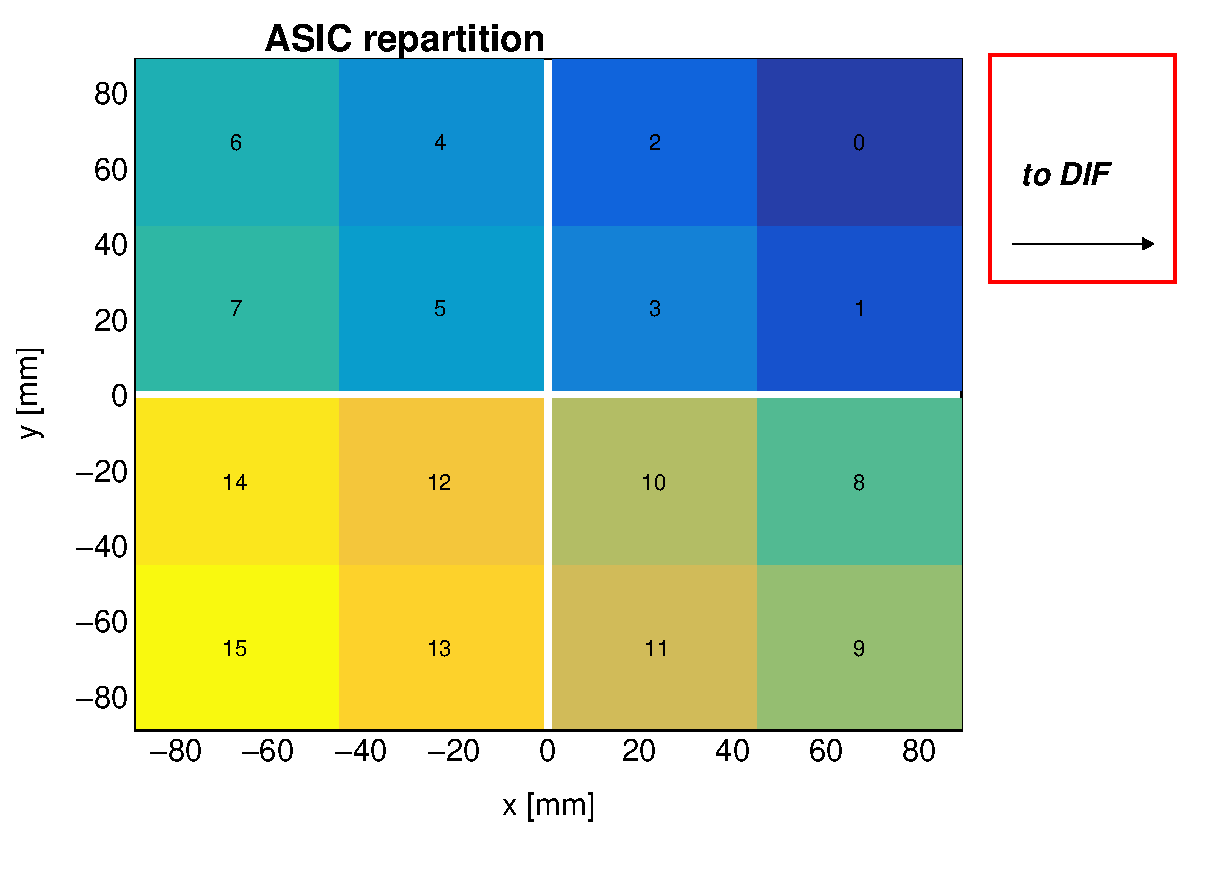
\includegraphics[width=4in]{../figs/ASU_geometry1.eps}  \\
    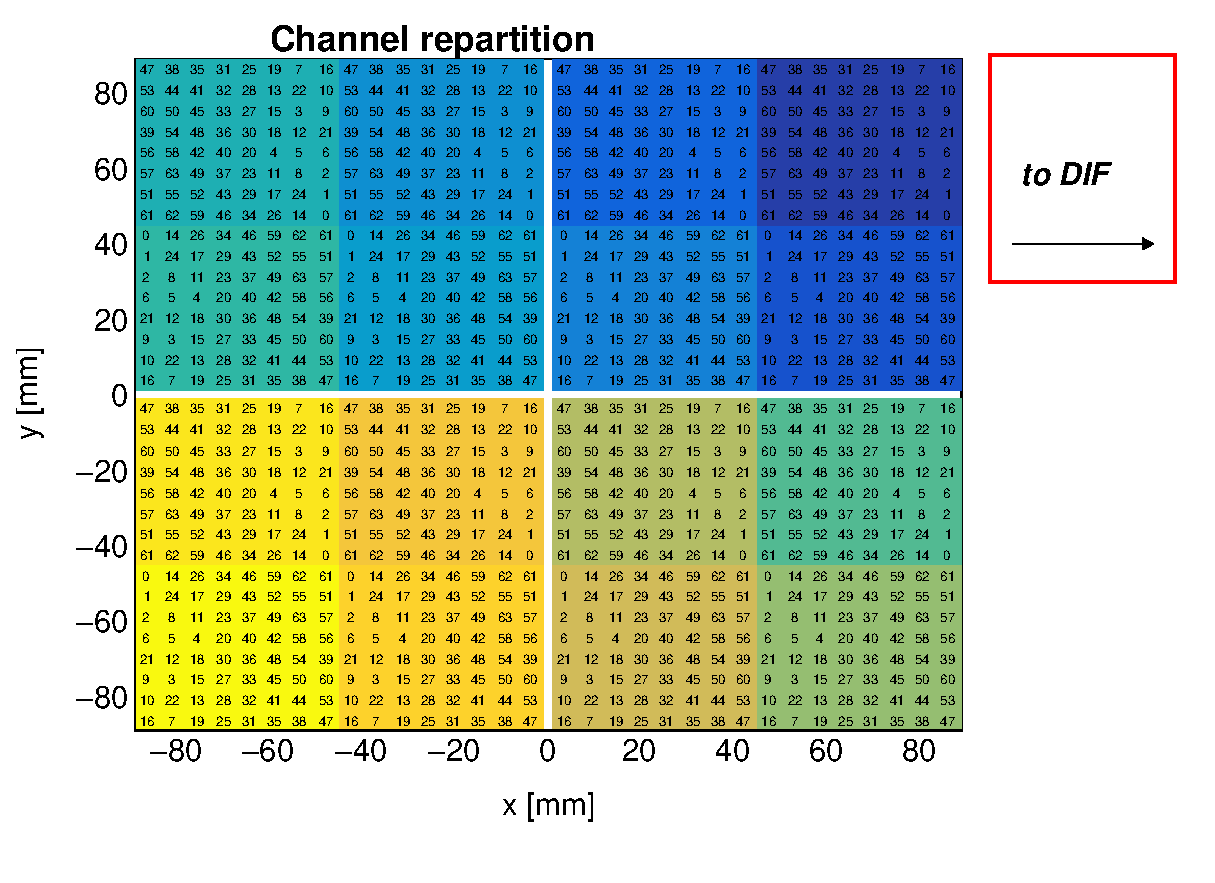
\includegraphics[width=4in]{../figs/ASU_geometry2.eps}  \\
  \end{tabular}
  \caption{Repartition of the ASIC (up) and channels (down) in one ASU. In this perspective, the Si-Sensors are in glued in the back.
    The channels are separated (in x and y) by 5.5 mm.
    The empty cross in the middle of the ASU corresponds to the 1 mm separation between the sensors.
    The areas covered by the different ASICs and channels
    are labeled with numbers following design and DAQ criteria: from 0-16 in the case of the ASICs and from 0-63 in the case of the channels.
  }
\label{ASU}
\end{figure}

The entity
of sensors, thin PCB (printed circuit boards) and ASICs is called Active Signal Units or ASU.
An individual ASU has a lateral dimension of 18x18 cm$^{2}$.
The ASUs are currently equipped
further with 16 SKIROC2 ASICs for the read out and features 1024 square pads (64 per ASIC) of 5x5 mm.
The channels and ASICs are distributed along the ASU as shown in Figure \ref{ASU}. Each ASU is equipped with 4 silicon wafers as the described in Section \ref{sec:wafers}.
The high voltage is delivered to the wafers using a HV-kapton sheet that covers the full extension of the wafers.

Current version of the PCB is called the FEV11. It has a thickness of 1.6mm and 2.7mm
if we include on top the ASICs in its current packaging (1.1 mm thick LFBGA package).
With these characteristics, a potential density of
3800 channels/dm$^{3}$ is achievable keeping the space and
interaction length requirements of the the baseline design of the ECAL forthe ILD.
This number should be compared with
the density achieved in beam tests with the physics prototype: 1500 channels/dm$^{3}$.
With the first versions
of the technological prototype we reached similar potential density level as in
the current version but equipping only a
quarter of the ASUs surface \cite{Amjad:2014tha}.

\subsection{Data AcQuisition system}
\label{sec:DAQ}

The subsequent chain of the data acquisition (DAQ)\cite{Gastaldi:2014vaa} system consists of three components, enumerate from upstream to downstream from the data flow perspective:

\begin{enumerate}
\item The first component is the so called detector interface (DIF) which is placed at the beginning of each layer holding up to 15 ASUs.
\item All DIFs are connected by single HDMI cables to the concentrator cards as the second component: the Gigabit Concentrator Cards (GDCCs). These cards are used to control up to 7 DIFs. They collect all data from the DIFs and distribute among them the system clock and fast commands.
  \item The most downstream component, is the clock and control card (CCC) which
provides a clock, control fan-out of up to 8 GDCCs and accepts and distributes external signals (i.e. signals
generated external pulse generator to simulate the ILC spill conditions).
\end{enumerate}

The whole system is controlled by the Calicoes and the Pyrame DAQ software version 3~\cite{Rubio-Roy:2017ere,Magniette:2018wdz}.

\subsection{Fully equipped readout modules: the SLABs}
\label{sec:setup}

\begin{figure}[!ht]
  \centering
    \includegraphics[width=6in]{../figs/short_slab_bga.jpg} 
  \caption{Open single SLAB with FEV11 ASU, 16 SKIROC 2 and the interface card visibles. }
\label{ASU2}
\end{figure}

A full equipped readout module is shown in Fig. \ref{ASU2}. These modules are called
SLABs and consist of a chain of one or several fully equipped ASUs
connected to a data acquisition system (DAQ) through an adapter board, called SMBv4.
The SMBv4 also serves as to hold other
services as power connectors or the super capacitances used for the power pulsing. 
These capacitances of 400mF with 16 m$\Omega$ of equivalent serial resistance. 
The capacitances are extra dimensioned to provide enough local storage 
of power to assure stable low voltage levels during the power pulsing. %In this configuration
%the high currents are still crossing the interconnections/
The readout modules are embedded on a "U" shape carbon structure to protect the wafers.
The full system is then covered by two aluminum plates
to provide electromagnetic shielding and mechanical stability.

For the production of the small sample of SLABs studied in this document,
a scalable working procedure has been established among several groups \cite{Boudry:2318814}
profiting from the funding of projects like AIDA2020 or the HIGHTEC emblematic project
of the P2IO. A schematic view of this assembly procedure chain can be seen in
Figure \ref{assembly}. For more details we refer to Ref.\cite{Boudry:2318814}.
This process is to be extrapolated to a full assembly procedure for
e.g. the ILD detector.

\begin{figure}[!t]
\centering
\begin{tabular}{l}
\includegraphics[width=4.0in]{../figs/assembly.png} 
\end{tabular}
\caption{Process flow for the assembly of the SiW-ECAL SLABs.}
\label{assembly}
\end{figure}

\subsection{The prototype setup}
\label{sec:setup2}

A picture showing the SiW-ECAL technological prototype setup can be seen in Figure \ref{proto}.
The current prototype consists on 7 layers of SLABs housed in a PVC and aluminum structure that can host up to 10 layers in slots separated by 15mm each.
The first six layers were placed in the first six slots and the last one was in the last slot, with respect to the beam. In the following sections, we will refer to layers number 1 to 7, where
the 1 is the closest to the beam pipe and 7 is the farthest.
This setup is used for commissioning (Section \ref{sec:commissioning}) and for the beam test
(Section \ref{sec:beamtest}). In both cases, the detector was
running in power pulsing mode. 

\begin{figure}[!ht]
\centering
\begin{tabular}{l}
\includegraphics[width=4.0in]{../figs/proto.png} 
\end{tabular}
\caption{Prototype with 7 layers inside the aluminum stack.}
\label{proto}
\end{figure}

\section{Commissioning}
\label{sec:commissioning}

This beam test was prepared by a commissioning phase comprising
the debug of the
short SLABSs with special emphasis in the control of the noise and the study of the
prototype performance in cosmic ray tests.

Earlier experiences with the SKIROC2 ASIC are reported in
Refs. \cite{Amjad:2014tha,Suehara:2018mqk}). 
Internal SKIROC2 parameters reported in these references are adopted in the following
unless stated otherwise.
For example, a gain value of 1.2pF for the preamplifier is used. 
With this gain, the SKIROC2 features a linearity better than 90\% 
for 0.5-200 MIPs, which is sufficient for 
electromagnetic showers created by few GeV 
electrons or positrons.

The main goal of the the commissioning  procedure is 
the optimization of the trigger thresholds to levels in which we are able
to record physics signals bellow the MIP level without saturating our DAQ with
noise signals. This requires a careful and systematic procedure to:

\begin{enumerate}
  \item identify the readout channels that are noisy in high trigger threshold above MIP signal conditions
  \item and select the optimal trigger threshold levels.
\end{enumerate}

During the commissioning, we observed the repetition of coherent noise events affecting to several
SLABs at the end of acquisitions with long gating time. The situation
could be remedied by improving the isolation of the individual SLABs and by reducing the
data taking to short gating times.

All runs dedicated to the commissioning were characterized by:
\begin{itemize}
  \item their short gating windows for the acquisition (1-2ms)
   at low repetition frequencies (1-5 Hz) to minimize the chances of having real events due to cosmic rays during the data taking and the coherent noise events due to grounding issues;
 \item and the relatively high trigger threshold values, between 2 and 0.5 MIPs.
\end{itemize}

\subsection{Tagging and control of the noisy channels.}
\label{sec:comm_noise}

We found to different types of noisy channels. One set consists of
channels randomly distributed along the surface of every ASU and the other consists
of channels located in specific areas and systematically noisy in all the ASUs. Preliminary inspections of the PCB layout
hint that the channels in the latter set may be noisy due to
improvable routing of the PCB.
Deeper studies on the PCB routing must be conducted to clarify this.
All the noisy channels have been identified and masked and the power
of their preamplifiers has been disabled. All the results shown in the following
sections are obtained in these conditions.

The list of the noisy channels was
obtained by means of dedicated data taking runs. In these runs
we scan trigger thresholds and progressively mask channels that exhibit counts. 
In each step, the decision of tagging a channel as noisy was taking following the next rules:

\begin{itemize}
\item if the channel was triggered at rates larger than 0.5-1\% of the total number of triggers per ASIC it was added to the list;
\item if a channel was tagged as noisy in, at least, three of the SLABs, it was tagged as noisy for all and added to the list of channels being suspect of suffer from routing issues.
\end{itemize}

In addition to the different noisy channel types described above, we also have
masked full sectors of the SLABs if an ASIC was faulty (at least 70\% of channels 
listed as noisy) or if a Si-wafer was damaged (high leakage currents).
The results of this study is summarized in Figure \ref{noisycells}.

\begin{figure}[!t]
  \centering
  \begin{tabular}{l}
  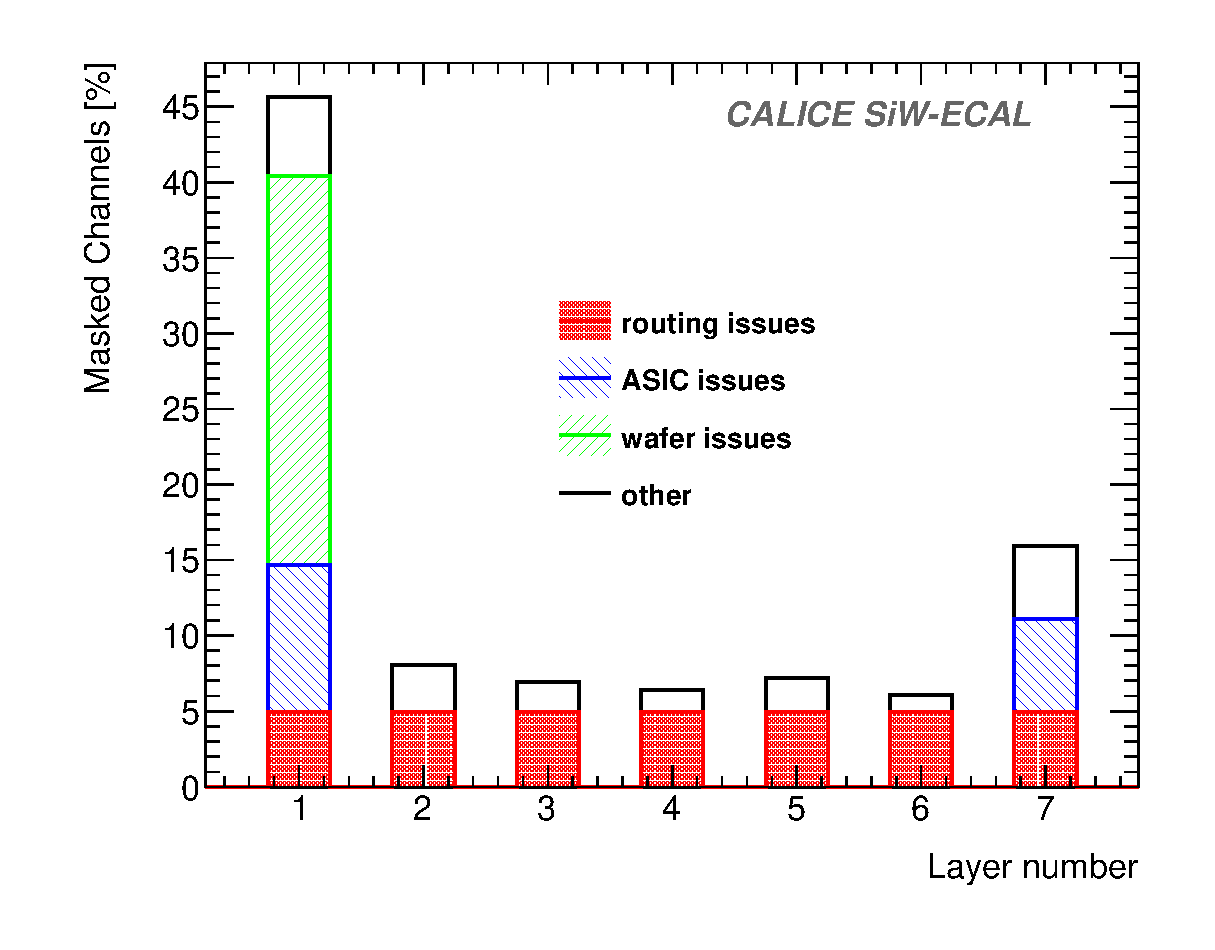
\includegraphics[width=4in]{../figs/commissioning/masked_layer.eps} \\
  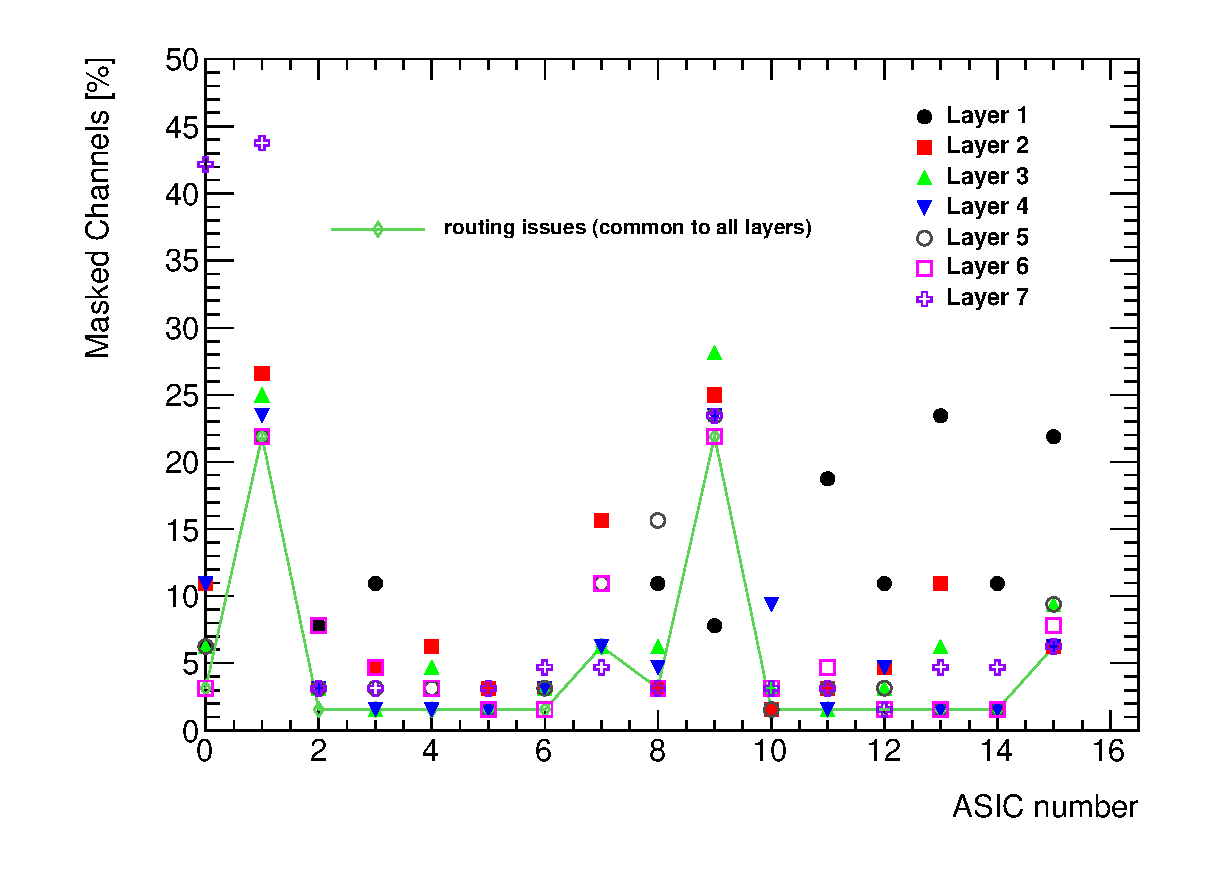
\includegraphics[width=4in]{../figs/commissioning/masked_chip.eps}
  \end{tabular}
\caption{Fraction of channels that are tagged as noisy in all slabs. 
Top: different type of noisy channels per slab. 
Bottom: break down of the total number of noisy channels per ASIC. 
The ASICs 4-7 (wafer issue) and 10 from layer 1 and the ASIC 4 from layer 7 are not included
in the second plot since they are fully masked.}
\label{noisycells}
\end{figure}


\subsection{Optimal trigger threshold determination}
\label{sec:comm_trigger}

After the noisy channels have been masked, dedicated trigger threshold
scan run are taken, and the results are shown in threshold scan curves where the
x-axis represents the threshold value and the y-axis
the number of recorded signals normalized to 1. The threshold values are given in internal DAC units
which are translated to meaningful physical quantities in Section \ref{sec:comm_trigger_sn}.
In the absence of external signals (cosmic rays, injected signals, etc) 
the falling edge position in the threshold scan curves
is due to the electronic noise
at the output of the fast shaper (the trigger decision branch on the SKIROC)
and it depends on the slow clock frequency.
These threshold scan curves are approximated by a complementary error function:

\begin{equation}
\frac{2p_{0}}{\sqrt(\pi)} \int_{\frac{DAC-p_{1}}{p_{2}}}^{\infty} e^{-t^{2}} dt,
\label{eq_S-curve}
\end{equation}
where $p_{0}$ is 1/2 of the normalization, $p_{1}$ is the value in which the noise levels are 
the 50\% of its maximum and $p_{2}$ give us the width of the threshold scan curve. 

In Figure \ref{scurve_channels} 
two threshold scans curves are shown together with the fit by
the theoretical function for two different channels from the second
layer of the setup are shown.

\begin{figure}[!ht]
  \centering
  \begin{tabular}{ll}
  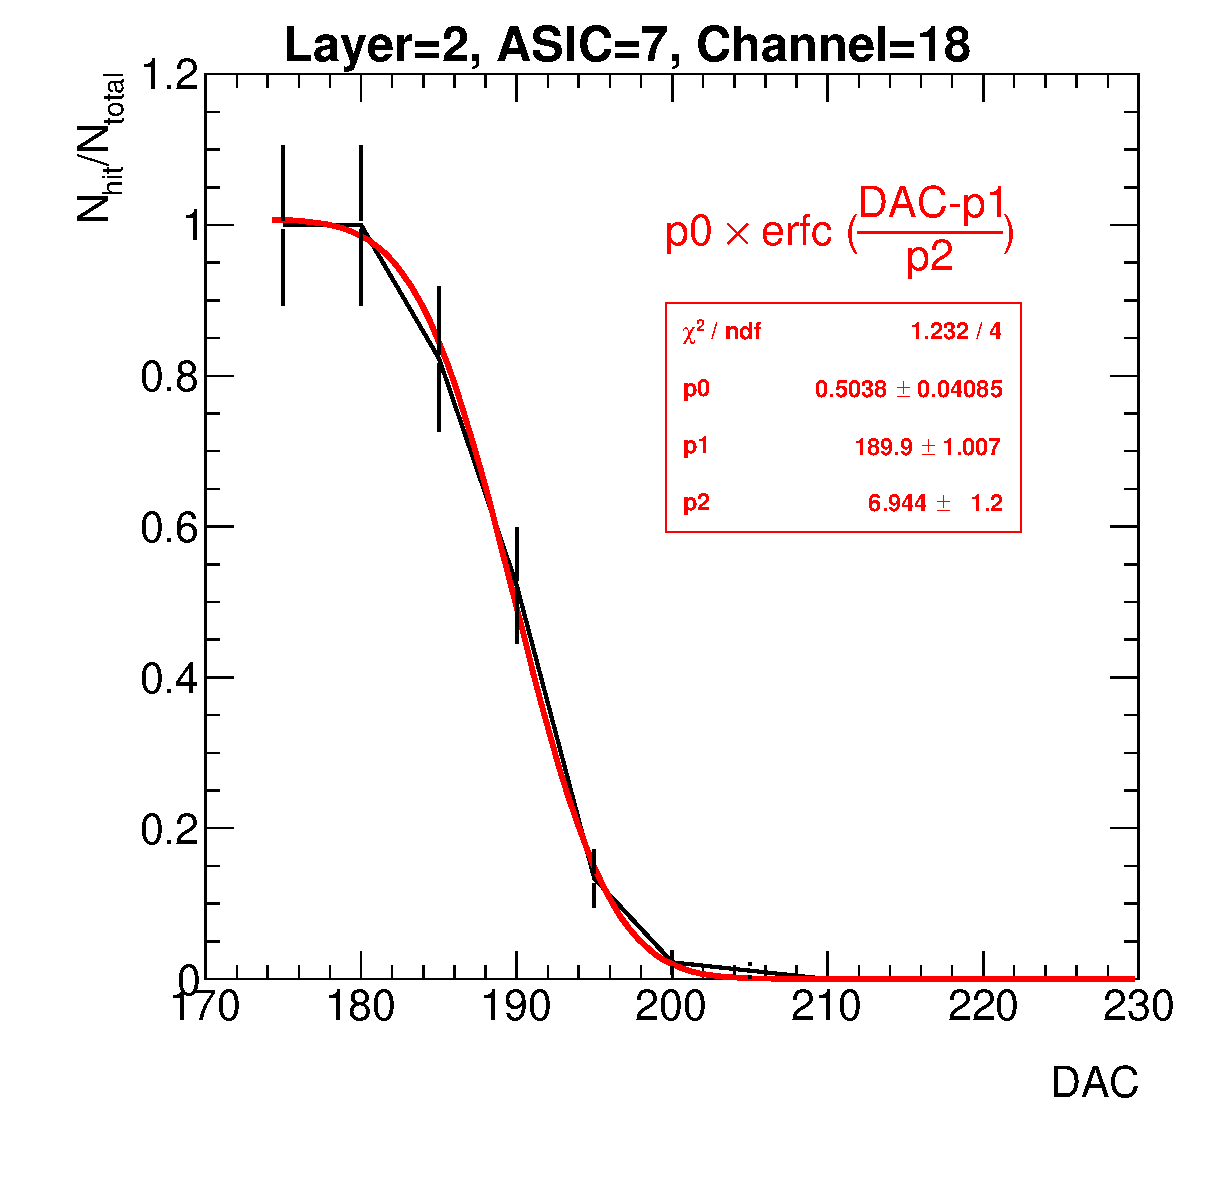
\includegraphics[width=2.8in]{../figs/commissioning/scurve_chn18_asic7_layer2.eps} & 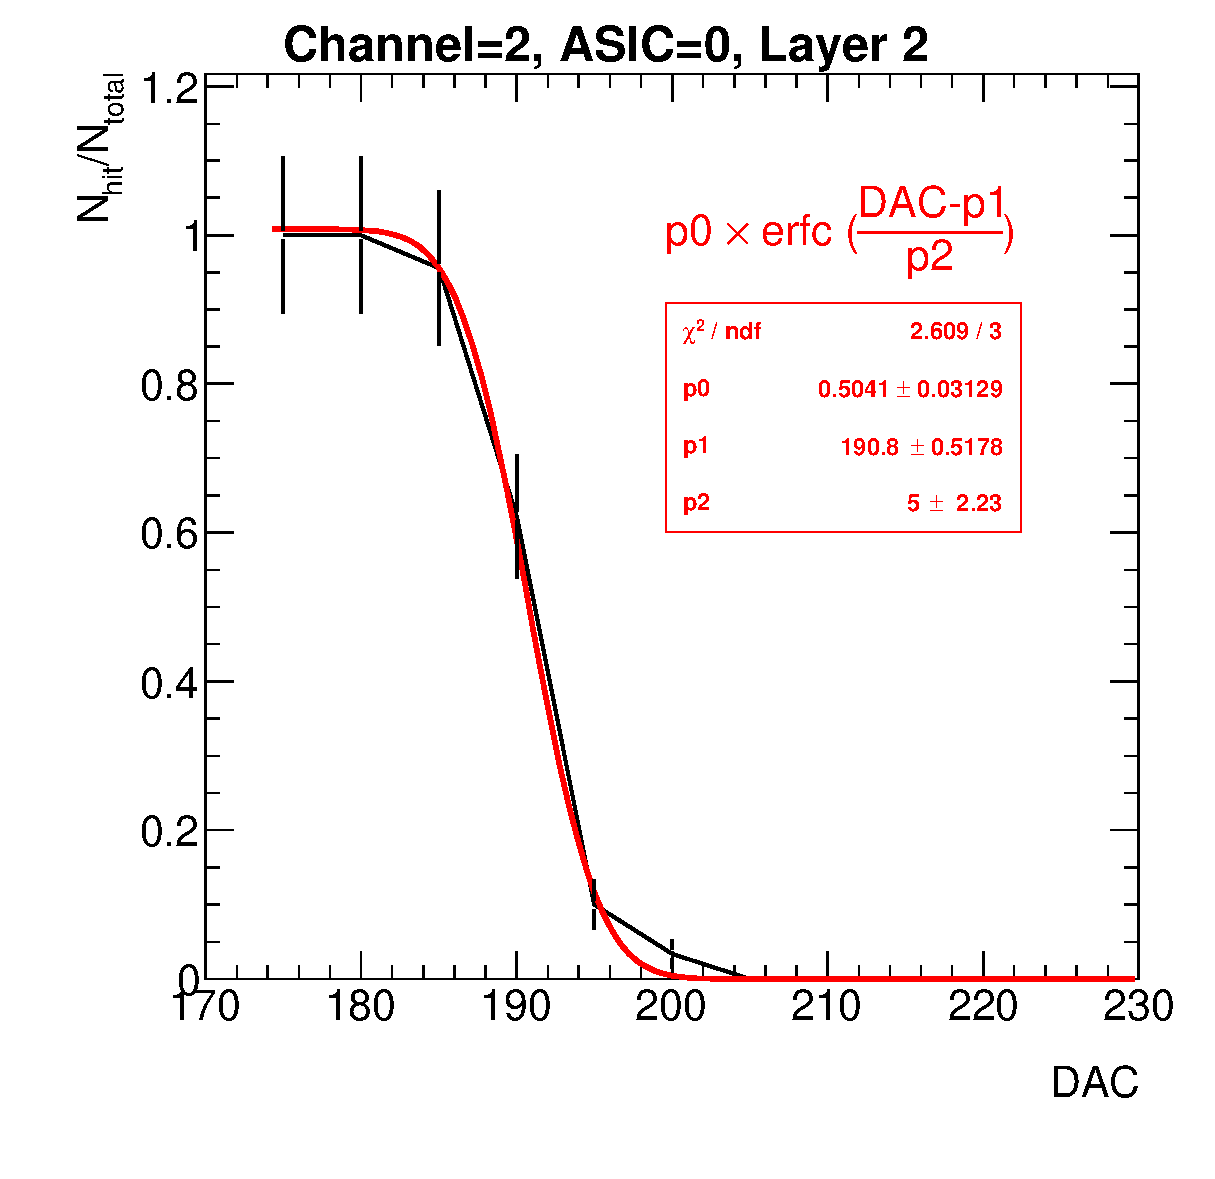
\includegraphics[width=2.8in]{../figs/commissioning/scurve_chn2_asic0_layer2.eps}
  \end{tabular}
\caption{Two threshold scan curves.}
\label{scurve_channels}
\end{figure}


For every ASICs, after performing the fit of the theoretical curves
to the threshold scans, the average values of the   $p_{1}$ and $p_{2}$ are calculated.
These are represented by $<p_{1,2}^{ASIC}>$ in the following.
The final threshold value of every ASIC, in DAC units, was chosen 
using the following formula
\begin{equation}
Threshold{optimal}^{ASIC} =maximum(<p_{1}^{ASIC}> + 5 \times <p_{2}^{ASIC}>,230).
\end{equation}
This formula was applied 
if at least the the 30\% of the 64 channels in the ASIC could be fitted.
If not, a global threshold value of 250 was set.

The optimal trigger threshold values for all ASICs are shown in Figure \ref{trigger_thresholds}, in internal DAC units and in MIPs. In the next section we explain how the conversion is done.

\subsection{S/N ratio in the trigger branch}
\label{sec:comm_trigger_sn}

Performing threshold scan scurves using
real signals allow to calculate the signal over noise (S/N) ratio to trigger.
For that we compare the curves for 1 MIP and 2 MIP injected signals.
The S/N is, therefore, defined as the ratio between the distance of both curves at its
50\% and the width of the curves.
In Figure \ref{scurves_injection} we see the 1 MIP and 2 MIP curves obtained for several channel
in a SKIROC testboard in which a single SKIROC2 in BGA package is placed and the 1 MIP and 2 MIPs 
 signals are directly injected in the preamplifier 
(via a 3 pF capacitor located in the injection line as shown in Figure \ref{SKIROC2}). 


\begin{figure}[!t]
    \centering
  \begin{tabular}{l}
	\includegraphics[width=4in]{../figs/commissioning/scurve_pp_fastshaper_ch_DAC.eps} \\
	\end{tabular}
\caption{Threshold scan curves with charge injection (1 MIP in blue and 2 MIPs in red) for two different channels in a SKIROC2 testboard.}
\label{scurves_injection}
\end{figure}


We have obtained similar results using real signals, in this case cosmic rays signals. This is shown 
in Figure \ref{scurves_cosmics}  where 
we show the result of the fit to the threshold scan curves cosmic rays integrated for all channels
in one ASIC. For completeness, the fit of threshold scan curves for all channels
in the same ASIC are also shown.

\begin{figure}[!ht]
    \centering
  \begin{tabular}{l}
	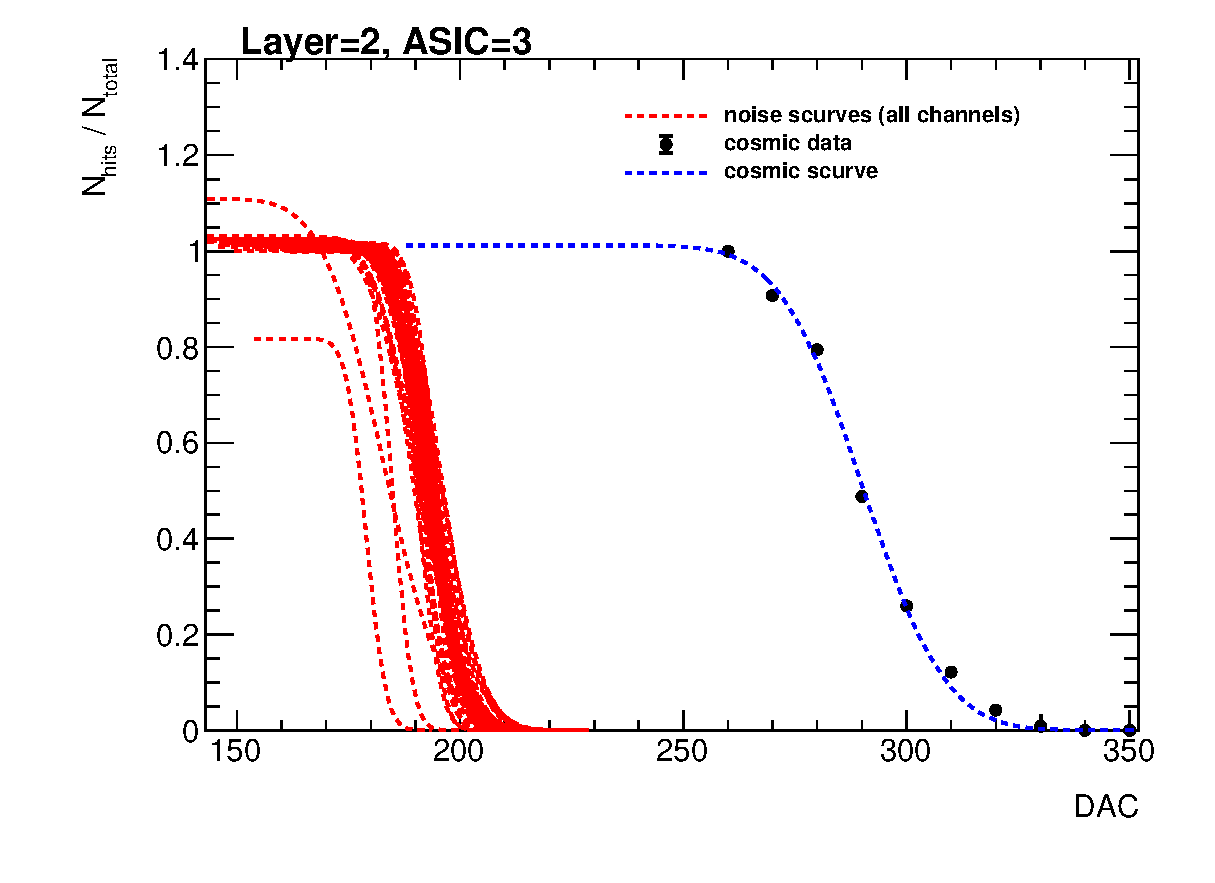
\includegraphics[width=4in]{../figs/commissioning/cosmic_scurves_asic3_layer2.eps} 
	\end{tabular}
\caption{Threshold scan curves for noise (channel by channel, only the result of the fit) and cosmic rays (all channels together) for one ASIC in layer 2.}
\label{scurves_cosmics}
\end{figure}

From these two results we extract the value of
\begin{equation}
  S/N=12.9\pm3.4
\end{equation}
for the trigger branch. The central value is calculated from the comparison of the blue and red curves
in Figure \ref{SKIROC2} and using the width of the 1 MIP curve in the denominator. The estimated
uncertainty has two components: the difference of width between the 1 and 2 MIP curves of injected signals and the differences (width and middle point) between the 1 MIP curves for injected and
cosmic ray signals.

Dedicated studies in beam test are needed in order to
reduce the uncertainty of this measurement.
However, by combining the information contained in the Figs \ref{scurves_injection} and \ref{scurves_cosmics}, we can also estimate the energy that corresponds
to a given trigger threshold.
This is shown in Figure \ref{trigger_thresholds}, where the chosen threholds of every ASIC being tested
in beam are shown.

\begin{figure}[!t]
  \centering
  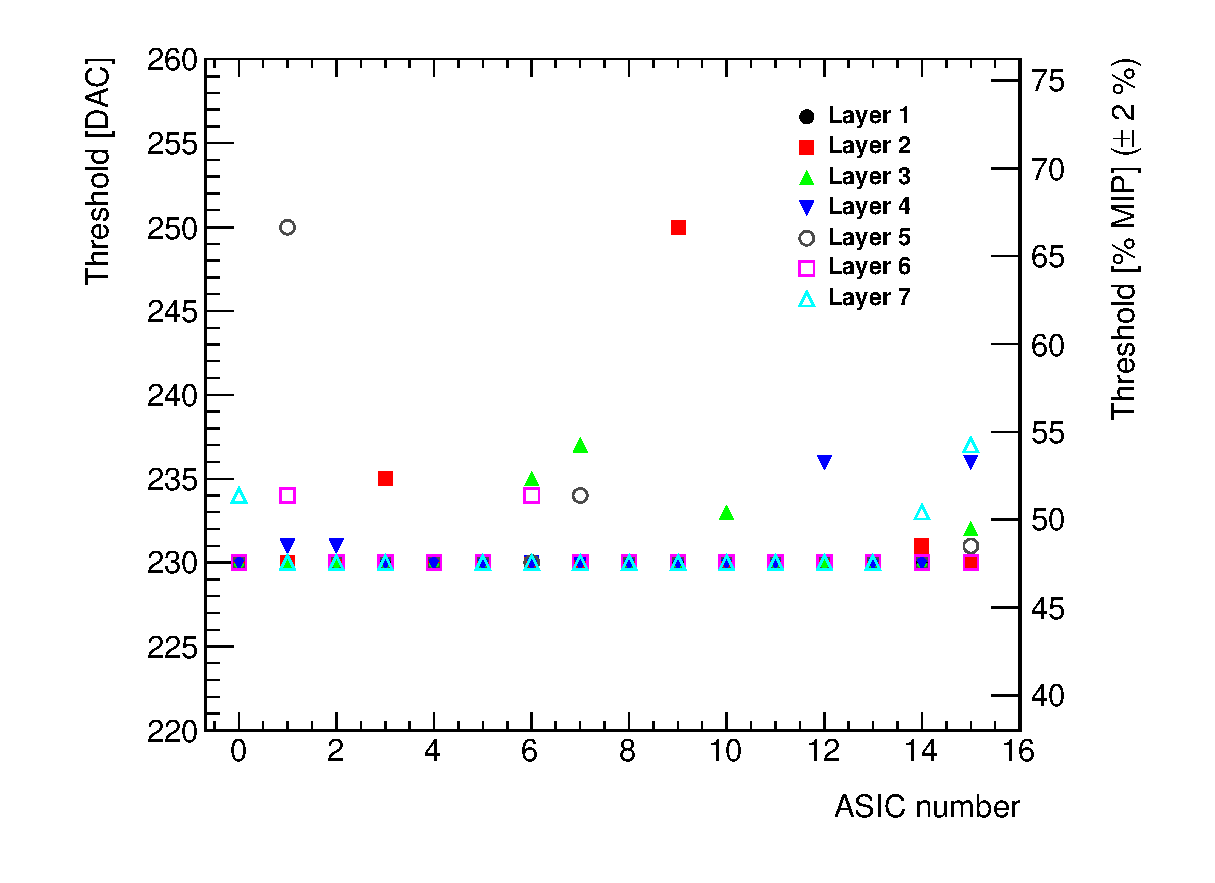
\includegraphics[width=4in]{../figs/commissioning/threshold_chip.eps}
  \caption{Summary of the trigger threshold settings in internal DAC units and in MIP units.}
\label{trigger_thresholds}
\end{figure}


\subsection{Prospects}
\label{sec:comm_prospects}

The commissioning procedure described above relies on very conservative decisions
due to the presence of unknown noise sources during largest of the commissioning phase.
These sources are
now well know and therefore a new ``noise commissioning procedure'' has been studied.
It will consist on an iterative algorithm that first
will identify and mask the channels
in which the number of triggers per channel will be compared with the number of expected triggers
assuming only cosmic rays as signal. This will allow us to have a
definition of the noise levels for each channel independently
instead of relative to the total number of triggers recorded by
the ASIC. Finally, once the noisy channels
are identified, the threshold  are further optimized
with a last run for the identification of the residual noisy channels.

Using this new procedure we manage to reduce the number of masked channels by a factor of two
without any loss of performance, at least in the laboratory and using 3 of the 7 SLABs.
This new procedure will also be applied in the next beam test.
Also, in order to
optimize the commissioning of the detector,
we propose a new set of measurements in the next beam test such as
a threshold scan for the determination of the S/N in the trigger line. The later
can be done by the comparison of threshold curves taken with incident MIP-acting particles
and MIP-acting particles traversing the detector tilted by 45 degrees with respect to the beam direction.


\section{Performance in a beam test with positrons at DESY}
\label{sec:beamtest}


The beam line at DESY provides continuous positron beams in the energy range of 1 to 6 GeV with
rates from a few hundreds of Hz to a few KHz with a maximum of $\sim 3$ KHz for 2-3 GeV. 
In addition, DESY gives access to a bore 1 T solenoid, the PCMag.

The physics program of the beam test can be summarized in the following points:

\begin{enumerate}
\item Calibration without tungsten absorber using 3 GeV positrons acting MIPs directed to 81 position equally distributed over the modules.
\item Test in magnetic field up to 1 T using the PCMag. For this test a special PVC structure was
  designed and produced to support one single SLAB.	
  The purpose of such test was twofold: first to prove that the DAQ, all electronic devices and the 
  mechanical consistency of the SLAB itself are able
  to handle strong magnetic fields; 
  second to check the quality of the data and the performance of the detector during the data taking when running
  in a magnetic field. 
  \item Response to electrons of different energies with fully equipped detector, i.e. sensitive parts {\it and} W absorber, with three different repartitions of the absorber material:
  \begin{itemize}
  \item W-configuration 1: $0.6,1.2,1.8,2.4,3.6,4.8$ and $6.6~X_{0}$
  \item W-configuration 2: $1.2,1.8,2.4,3.6,4.8,6.6$ and $8.4~X_{0}$
  \item W-configuration 3: $1.8,2.4,3.6,4.8,6.6,8.4$ and $10.2~X_{0}$
  \end{itemize}
\end{enumerate}

First reports on this beam test can be find in
Refs. \cite{Irles:2018uum,Irles:2018hcd}. These results have extended and
are discussed in the following sections. In Section \ref{sec:calib} we discuss in detail
the results of the pedestal, noise and MIP calibration.
We show also results on the pedestal and noise stability when running inside
a magnetic field in Section \ref{sec:magnetic} and in electromagnetic shower
events in Section \ref{sec:showers}. The study of the calibration of the prototype
in electromagnetic shower events is due to a future publication.

\subsection{Noise studies and MIP calibration}
\label{sec:calib}

In Figure \ref{signal_pedestal} we show the signal and pedestal distribution of a single channel after
subtracting the pedestal mean position. The results of the MIP calibration fit are shown in red.
The signal distribution is integrated over all SCAs.
For cosmetic reasons the pedestal distribution is shown only for the first SCA.

%\subsubsection{Pedestal and noise determination}
%\label{sec:pedestal}

\begin{figure}[!ht]
  \centering
  \begin{tabular}{l}
    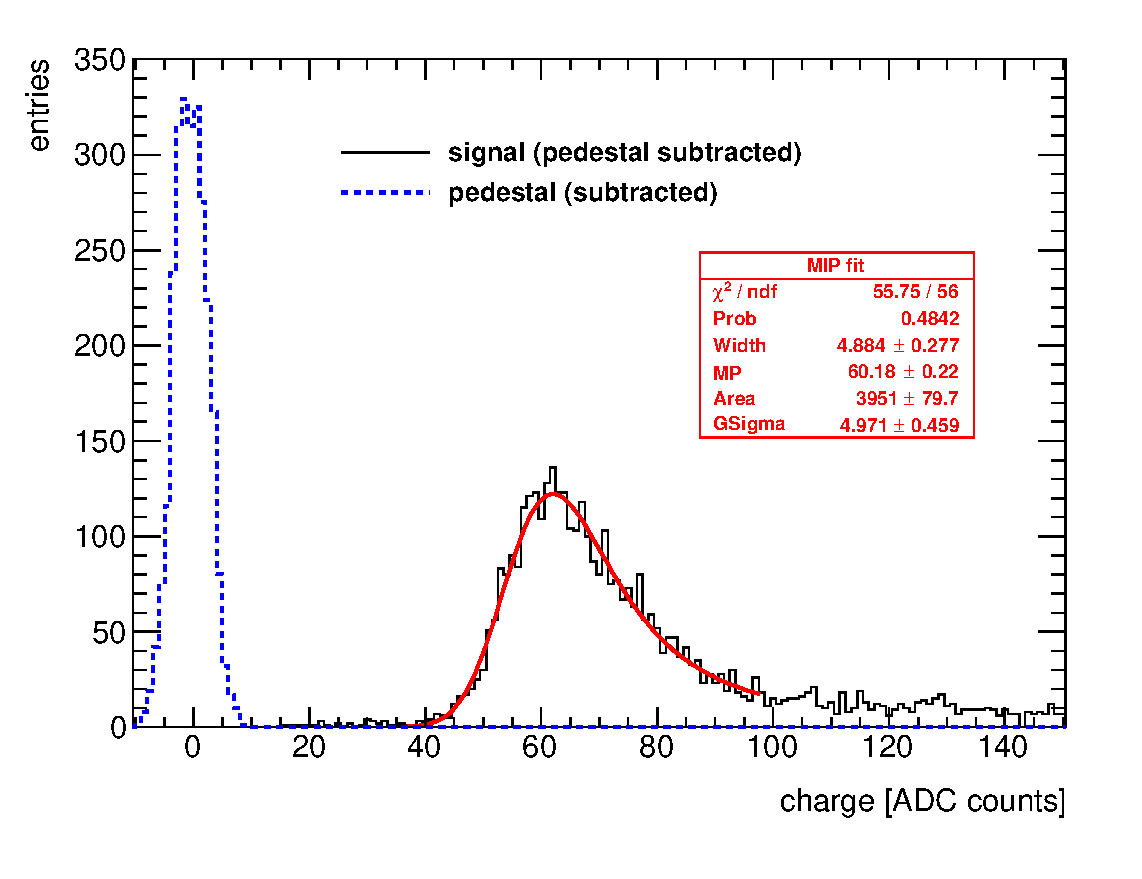
\includegraphics[width=4in]{../figs/mip_pedestal_example.eps}
  \end{tabular}
  \caption{Pedestal (blue dashed line) and signal (black continuous line) distribution for one channel in the third layer.}
\label{signal_pedestal}
\end{figure}

The pedestal is calculated as the mean position of
the distribution of the ADC values for all channels without trigger. The noise is
associated to the width of the distribution.
The pedestal correction is done layer-, chip-, channel- and SCA-wise due to the large spread of values between pedestals, as observed in 
Figure \ref{pedestal_layer} (left plot) and Figure \ref{pedestal_all} (also left plot).
For the noise, the dispersion is much smaller ($\sim 5 \%$). This is shown in the right plots of Figures \ref{pedestal_layer} and \ref{pedestal_all}.
From now on, the pedestal correction is applied to all the results presented.
The resulting spectra are fit by
a Landau function convoluted with a Gaussian.
The most-probable-value of the convoluted function is taken as the MIP value, allowing thus for a direct
conversion from ADC units to energy in MIP units.
The fit succeeded in 98\% of the cases and the spread of the resulting MPV is 5\%.
The remaining channels will be discarded. Results are summarized in figure \ref{mipandSN}, leftmost plot.

\begin{figure}[!t]
  \centering
  \begin{tabular}{ll}
    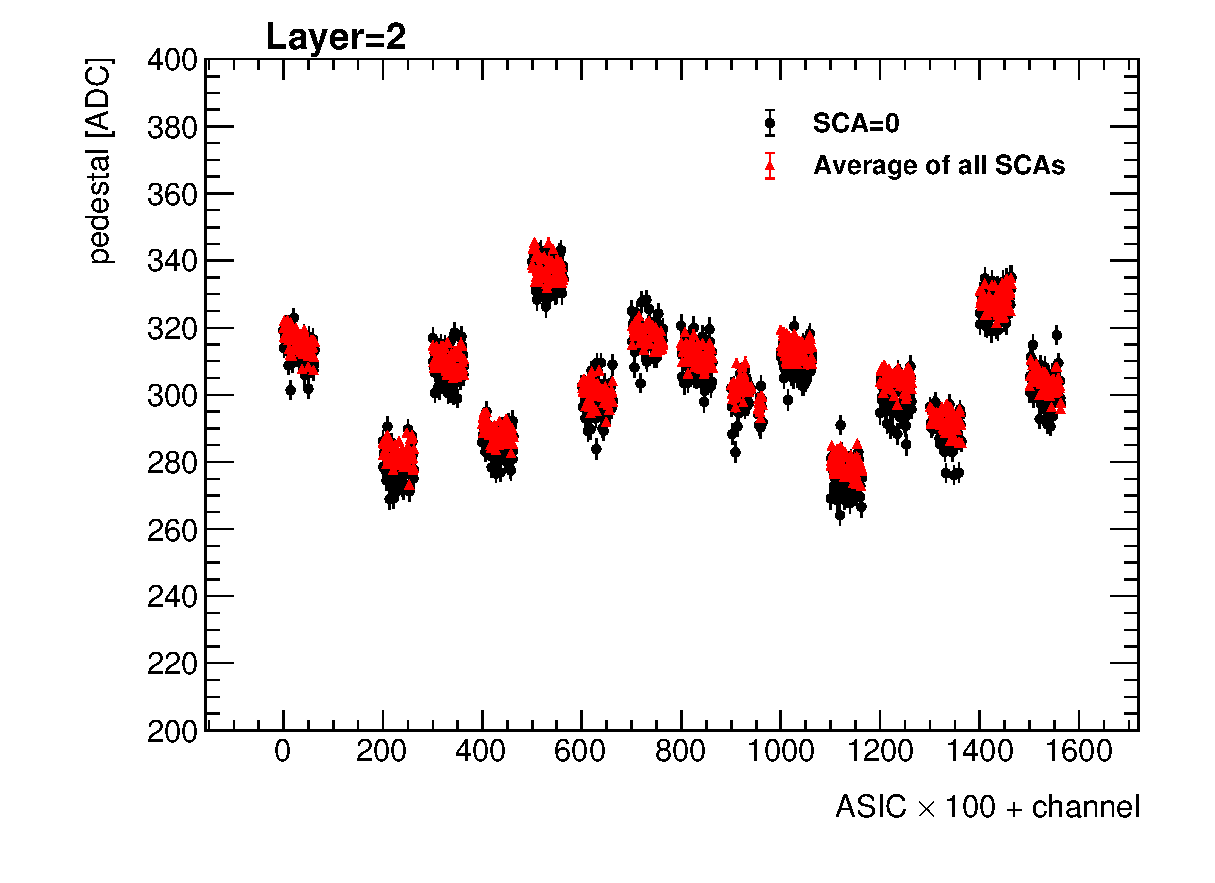
\includegraphics[width=2.8in]{../figs/pedestal/ped_mean_layer2.eps} & 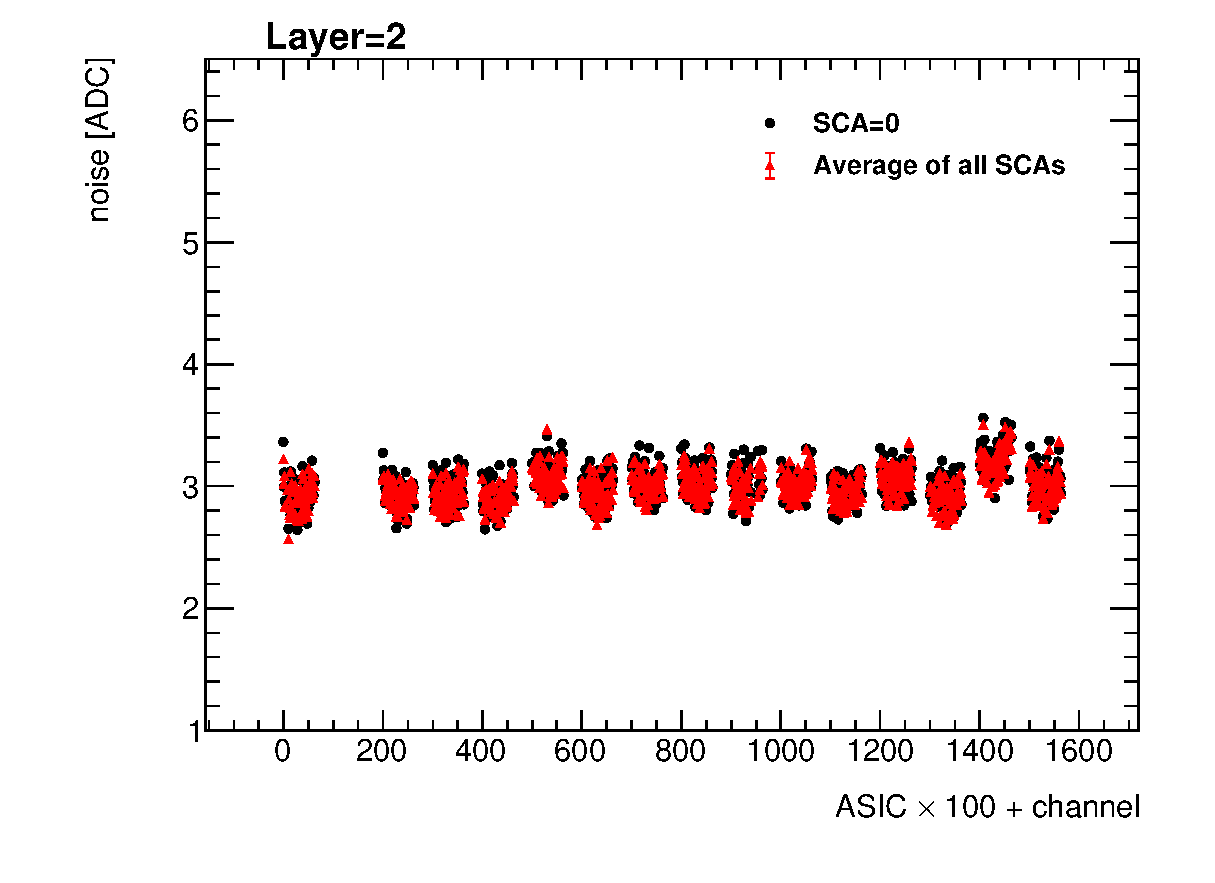
\includegraphics[width=2.8in]{../figs/pedestal/width_mean_layer2.eps}
  \end{tabular}
  \caption{Pedestal mean position (left plot) and width (right plot) for all channels in one layer.}
\label{pedestal_layer}
\end{figure}

\begin{figure}[!t]
  \centering
  \begin{tabular}{ll}
    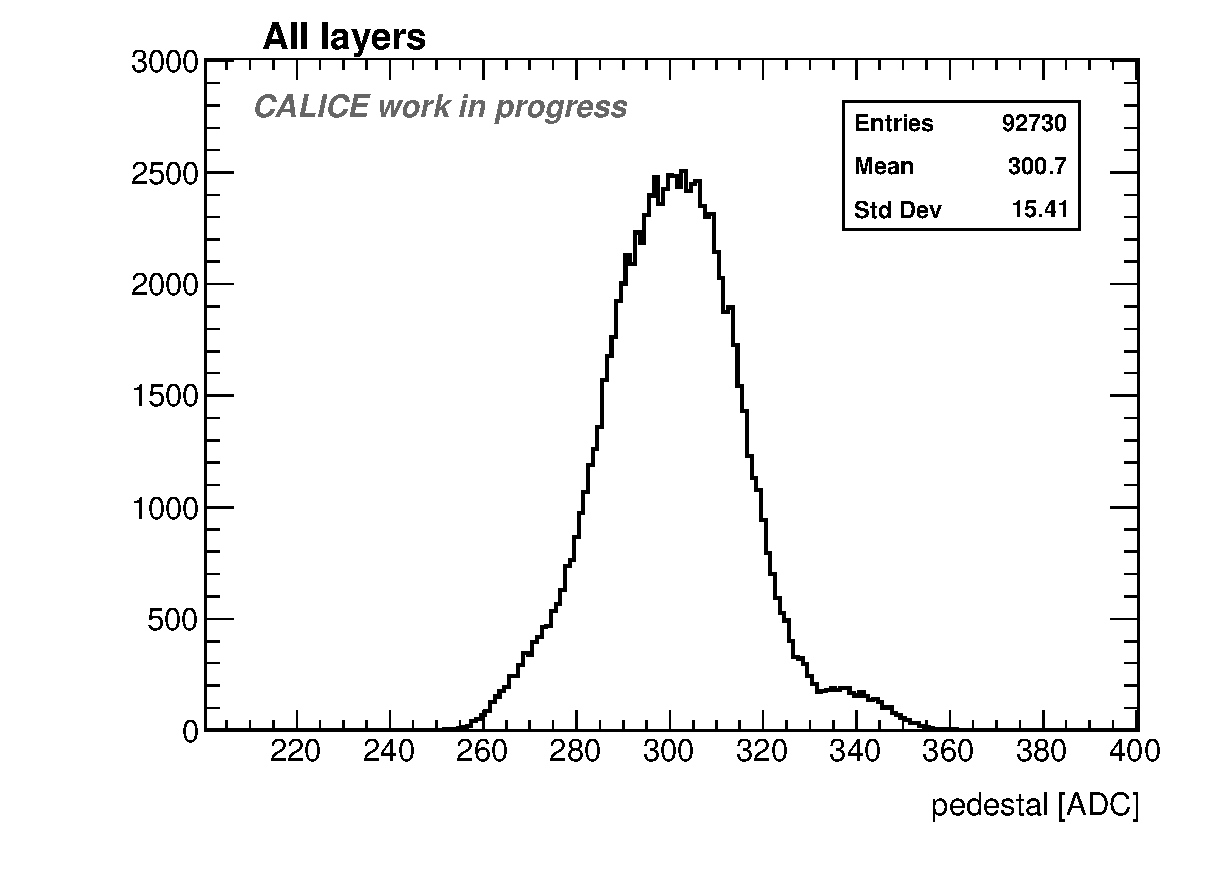
\includegraphics[width=2.8in]{../figs/pedestal/h_ped_mean.eps} & \includegraphics[width=2.8in]{../figs/pedestal/h_ped_width.eps}
  \end{tabular}
  \caption{Pedestal mean position (left) and width (right) for all channels and all SCAs in the setup.}
\label{pedestal_all}
\end{figure}


\begin{figure}[!t]
  \centering
  \begin{tabular}{ll}
      \includegraphics[width=2.8in]{../figs/MIP/MIPsummary_title.eps} & \includegraphics[width=2.8in]{../figs/MIP/SNsummary_title.eps}  
  \end{tabular}
\caption{Result of the MIP position calculation and signal over noise calculation for all calibrated channels.}
\label{mipandSN}
\end{figure}

As a sumamry Figure \ref{mip3peaks} shows the response of all channels integrated over the calibration run.
This plot is obtained after further refinement of the sample by selecting incident tracks.
The maximum peaks at 1 MIP as expected after a good calibration.
In addition to this, a second and a third peaks
are visible as shoulders. These shoulder are associated to 
events involving multiple 
particles crossing the detector.

\begin{figure}[!t]
  \centering 
    \begin{tabular}{ll}
      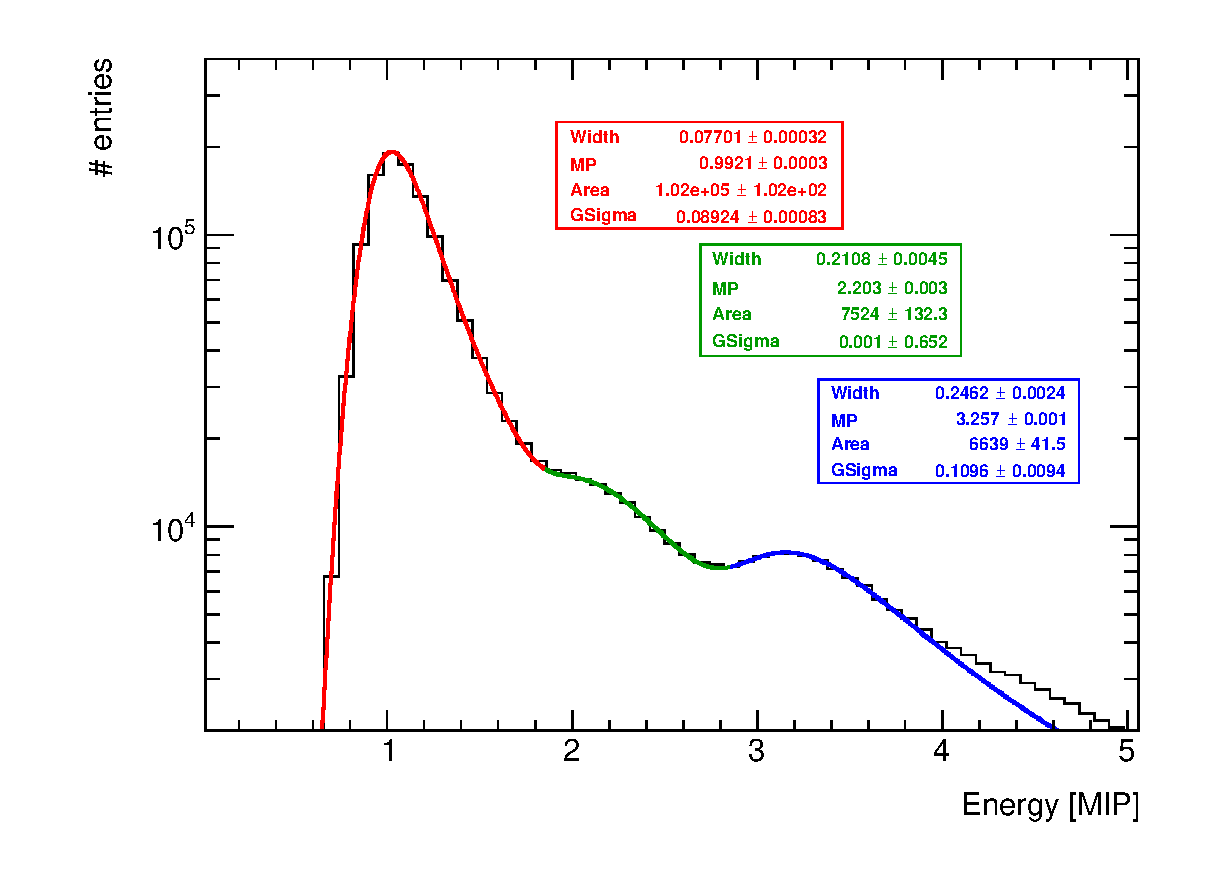
\includegraphics[width=4in]{../figs/MIP/MIP3peaks.eps} 
    \end{tabular}
    \caption{Energy distribution for all calibrated channels when selecting incident tracks of 3 GeV positron acting as MIPs.}
\label{mip3peaks}
\end{figure}

To evaluate 
the single hit detection efficiency we define a high purity sample of
events by selecting
tracks with at least 4 layers with a hit in exactly the same channel. Afterwards we 
check which layers have or not a hit in the same or in the closest neighboring channels with energy larger or equal than 0.3 MIP.
We repeat this procedure for all channels.
The results are shown in Figure \ref{efficiency}. Except few exceptions, the efficiency is 
compatible with $100\%$.
Lower efficiencies in the first layer are related to the presence of
noisy channels not spotted during the commissioning. In the last layer we also observe few small deviations
which are associated to the outliers channels, hinting for a small misalignment of the last layer.

\begin{figure}[!t]
  \centering 
   % \begin{tabular}{ll}
  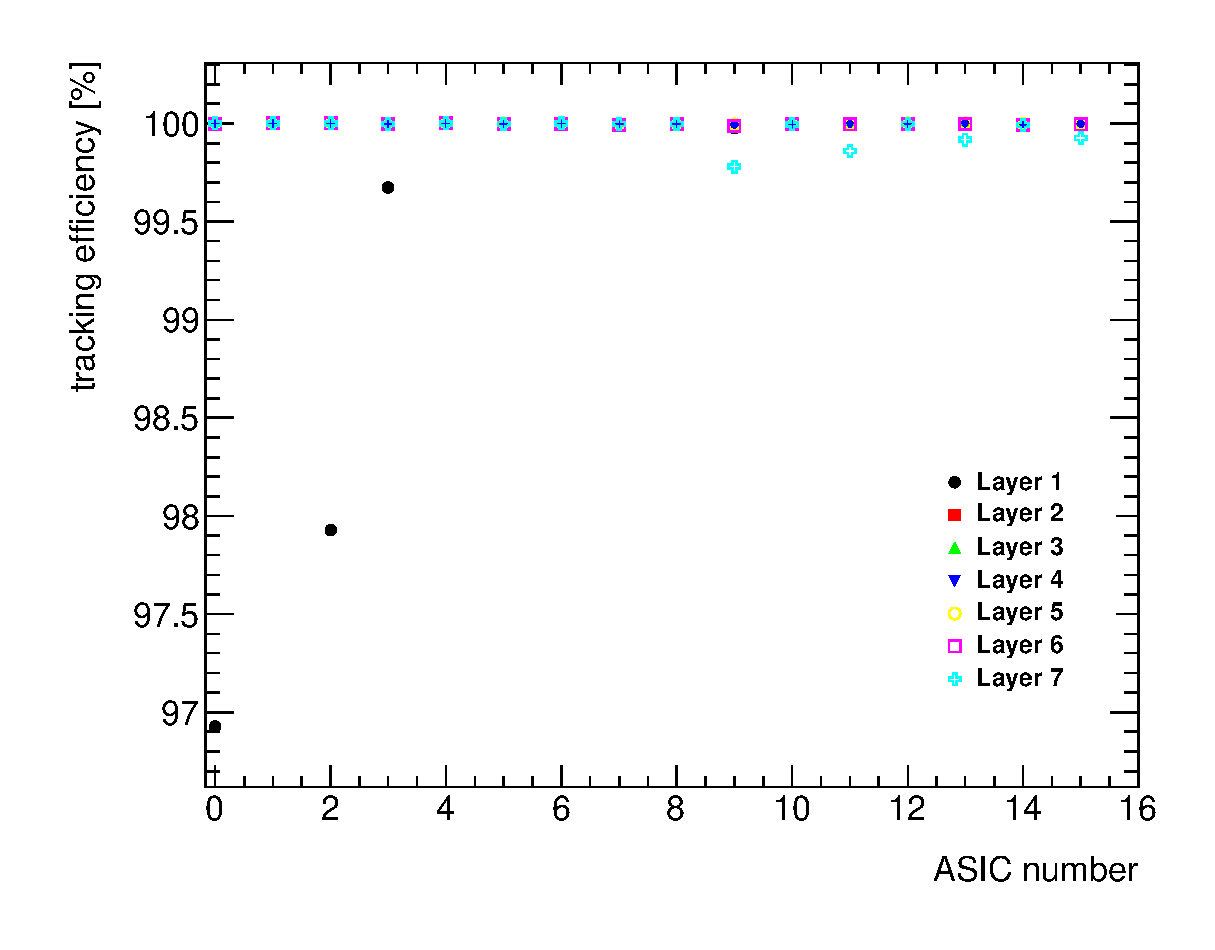
\includegraphics[width=4in]{../figs/MIP/efficiency_nhits4_chips.eps}
  %& 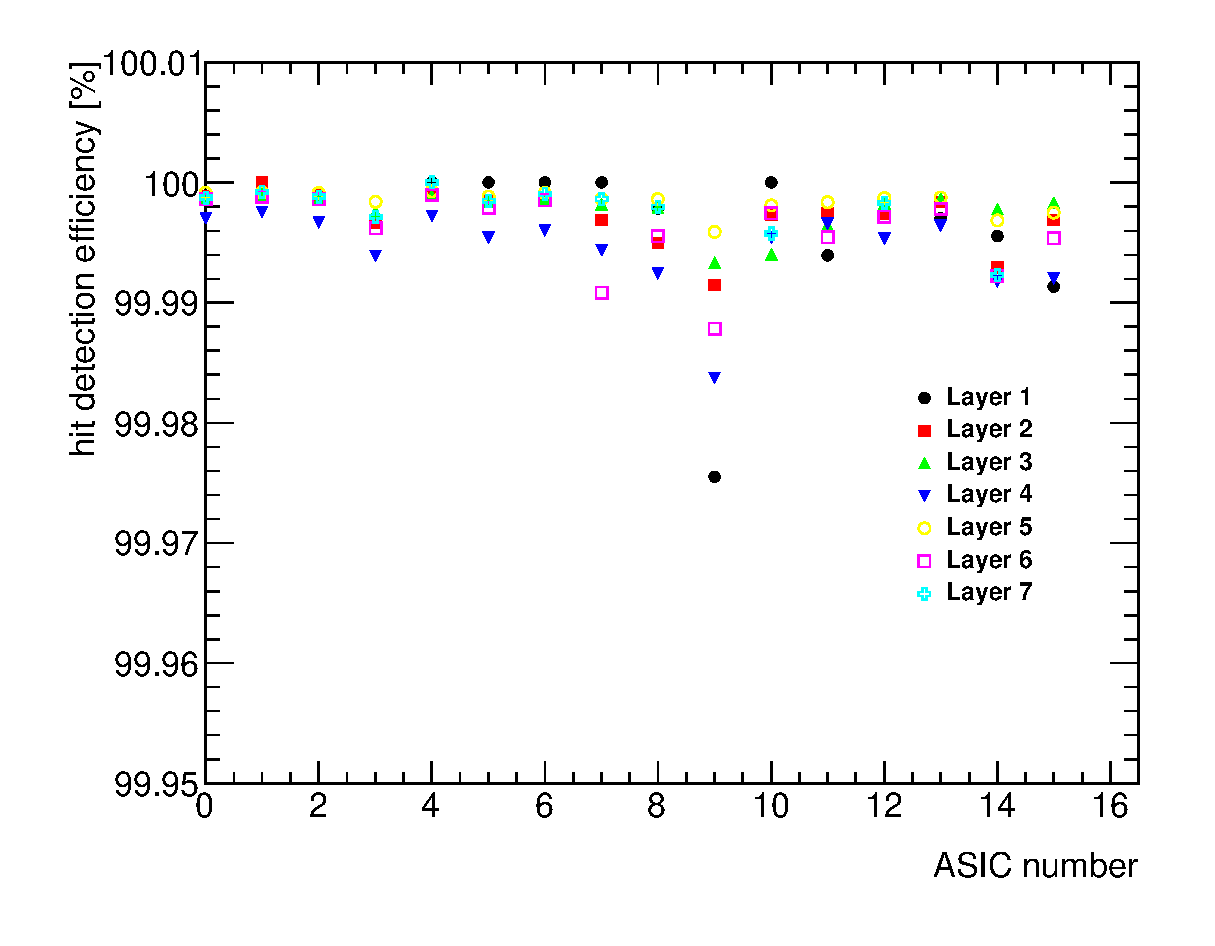
\includegraphics[width=2.8in]{../figs/MIP/efficiency_nhits4_chips_zoom.eps} \\
  %  \end{tabular}
  \caption{MIP detection efficiency for all layers and ASICs in high purity samples of tracks of MIP-like acting particles.}
\label{efficiency}
\end{figure}


\subsubsection{S/N ratio in the charge measurement for MIP interactions}
\label{sec:sn}

The signal-over-noise ratio in the charge measurement (corresponding to the slow shaper of the SKIROC2) is defined 
as the ratio between the most-probable-value of
the Landau-gauss function fit to the data (pedestal subtracted) and the noise (the pedestal width). This quantity 
has been calculated for all channels and all layers. 
Results are summarized in Figure \ref{mipandSN}, rightmost plot.

\subsection{Pedestal and noise stability in a magnetic field}
\label{sec:magnetic}

The data taking inside the magnetic field has been divided in three runs:
\begin{enumerate}
\item a with a magnetic field of 1 T;
\item a run with 0.5 T;
\item and a final run with the magnet off.
\end{enumerate}

The beam, 3 GeV positrons, was directed in the area of the PCB readout by the ASIC number 12.
The pedestal positions and noise levels of the channels of the ASIC 12 when the
SLAB is inside of the PCMag are compared with the results from the calibration run described in the previous section.
This is shown in Figure \ref{pedestal_magnetic}.
We see that the agreement is perfectly good within the statistical uncertainties.
Due to the lower rates in this beam area, the
analysis is only done up to few SCAs.

\begin{figure}[!t]
  \centering
  \begin{tabular}{ll}
    \includegraphics[width=2.8in]{../figs/pedestal/1T/summary_pedestal_chip12.eps} & \includegraphics[width=2.8in]{../figs/pedestal/1T/summary_noise_chip12.eps}
  \end{tabular}
  \caption{Average deviation of the pedestal mean position (left) and width (right) for all channels in the ASIC 12.}
\label{pedestal_magnetic}
\end{figure}

\subsection{Pedestal stability in electromagnetic shower events}
\label{sec:showers}

In this section we discuss the pedestal stability in events with large amount of charge collected by the ASICs, as are the 
electromagnetic shower events. All the results shown in this section correspond to data taken during the tungsten program, 
using the W-configuration number 2 when shooting the beam in the area registered by the ASIC 12 (and partially in the 13). 
For simplicity, only information recorded by ASIC 12 will be shown. 
In order to select a high purity of
electromagnetic shower like the events, 
we used a simple criteria: select only events with at least 6 of the layers with at least a hit with E > 0.5 MIP.

\begin{figure}[!ht]
  \centering 
    \begin{tabular}{ll}
      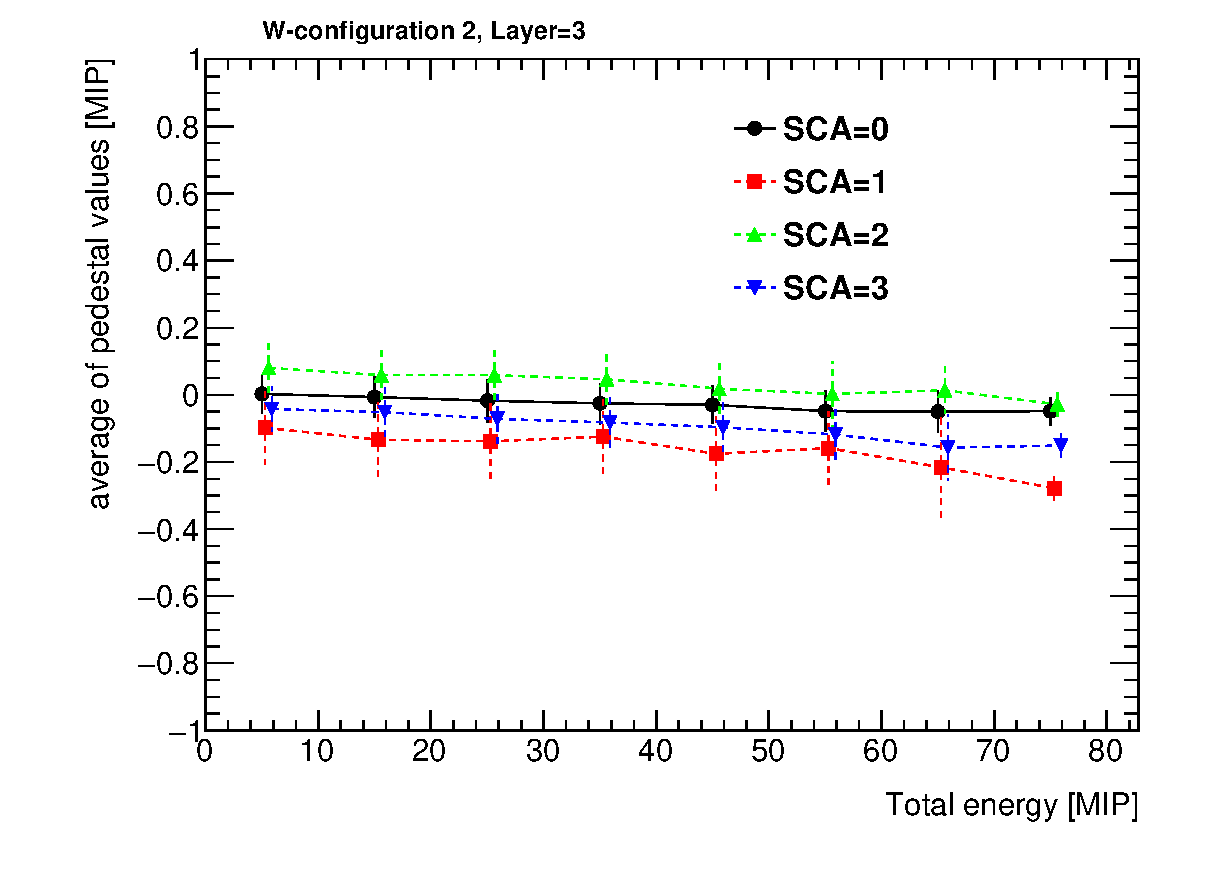
\includegraphics[width=2.8in]{../figs/pedestal/pedestal_vs_energy_shower.eps} & 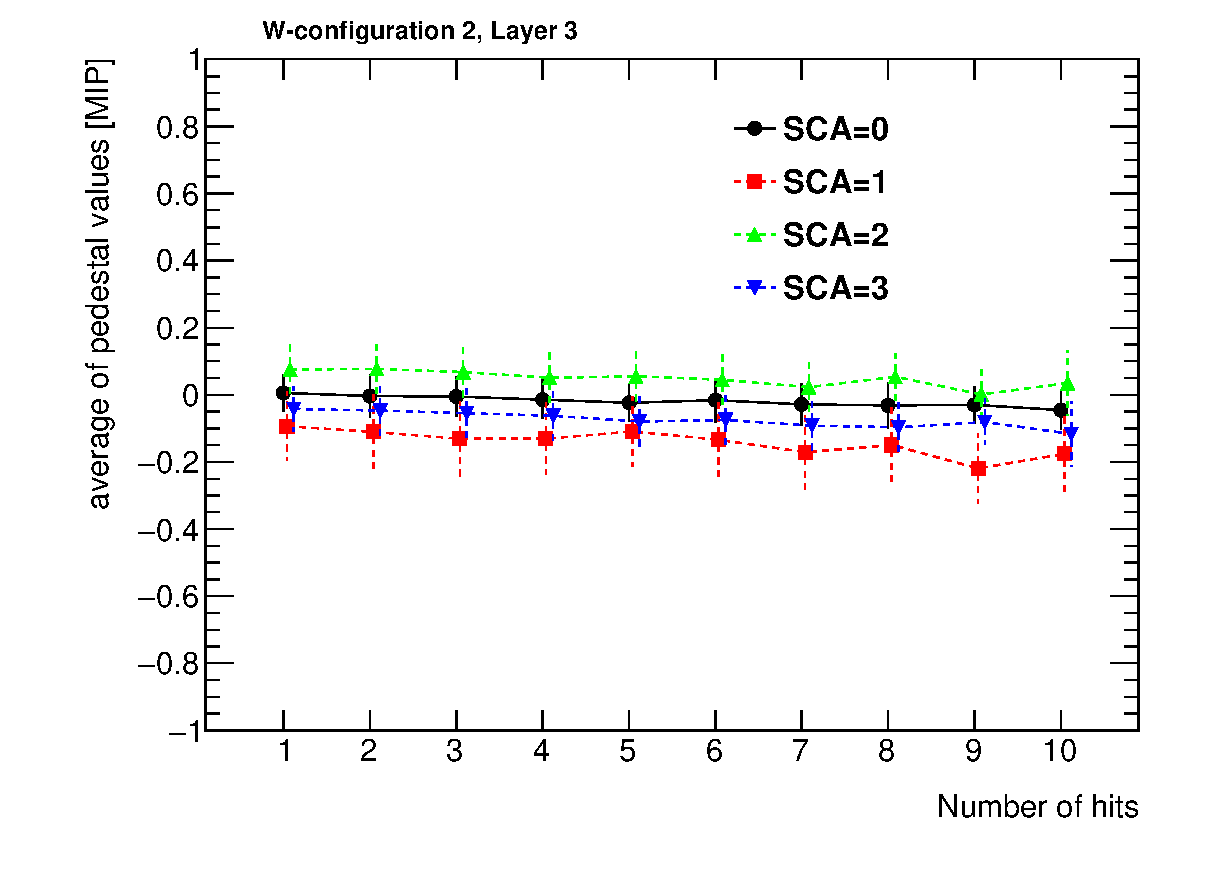
\includegraphics[width=2.8in]{../figs/pedestal/pedestal_vs_nhits_shower.eps} \\
    \end{tabular}
    \caption{Left: mean position of the projection of the pedestal distribution of all channels
      calculated when different energies are collected in the ASIC (in bins of 10 MIPs).
      Right: same but as a function of the number of hits. In both cases, the results are shown for few SCA.
      The points for the curves with SCA different than zero are slightly shifted in the x-axis to optimize the visualization.}
\label{pedestal_shower_1}
\end{figure}

Two main observations have been extracted from the recalculation of the pedestals and its comparison
with the values obtained previously during the calibration runs. The first observation
consists in a relatively small 
drift of the pedestal values
towards lower values when the collected energy is high {\it i.e.} when the number of triggered channels is large.
This is shown in Figure \ref{pedestal_shower_1} for several SCAs.
A small dependence, in all SCAs, of the pedestal position on the amount of charge collected by the
ASIC is observed.
This feature is known and it is due to the architecture of the SKIROC2 ASICs 
where high inrush of currents can slightly shift the baseline of the analogue power supply. 
The second observation extracted from this analysis can be also seen in Figure \ref{pedestal_shower_1} but
more clearly in Figure \ref{pedestal_shower_2}: in addition
to the small drift of the pedestal value an SCA-alternate global shift
is observed. We see that the effect is enhanced when large amounts of charge
are deposited in the ASIC ({\it i.e.} at larger beam energies or for the layers in the maximum of the shower
profile). We also observed that this alternation is only SCA dependent and does not depends
on the time in which the deposit of energy occurs within the acquisition.
This is not yet fully understood although the fact that the effect is observed in
alternate SCAs hints that something is affecting to the digital part of the ASIC 
(where the SCAs enter in play).
Dedicated tests in the laboratory and in the beam are needed in order to clarify this issue.

\begin{figure}[!t]
  \centering 
    \begin{tabular}{ll}
      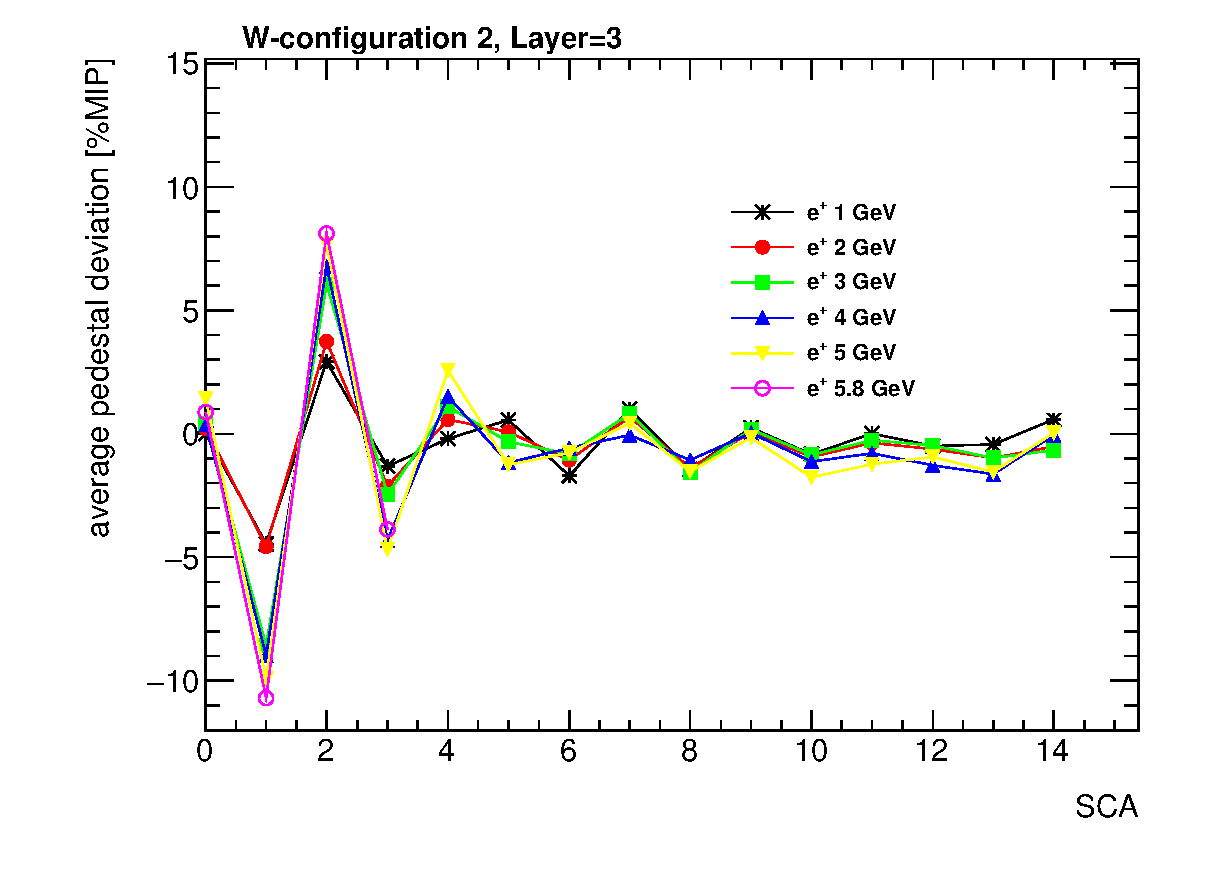
\includegraphics[width=2.8in]{../figs/pedestal/pedestal_deviation_layer3.eps} & 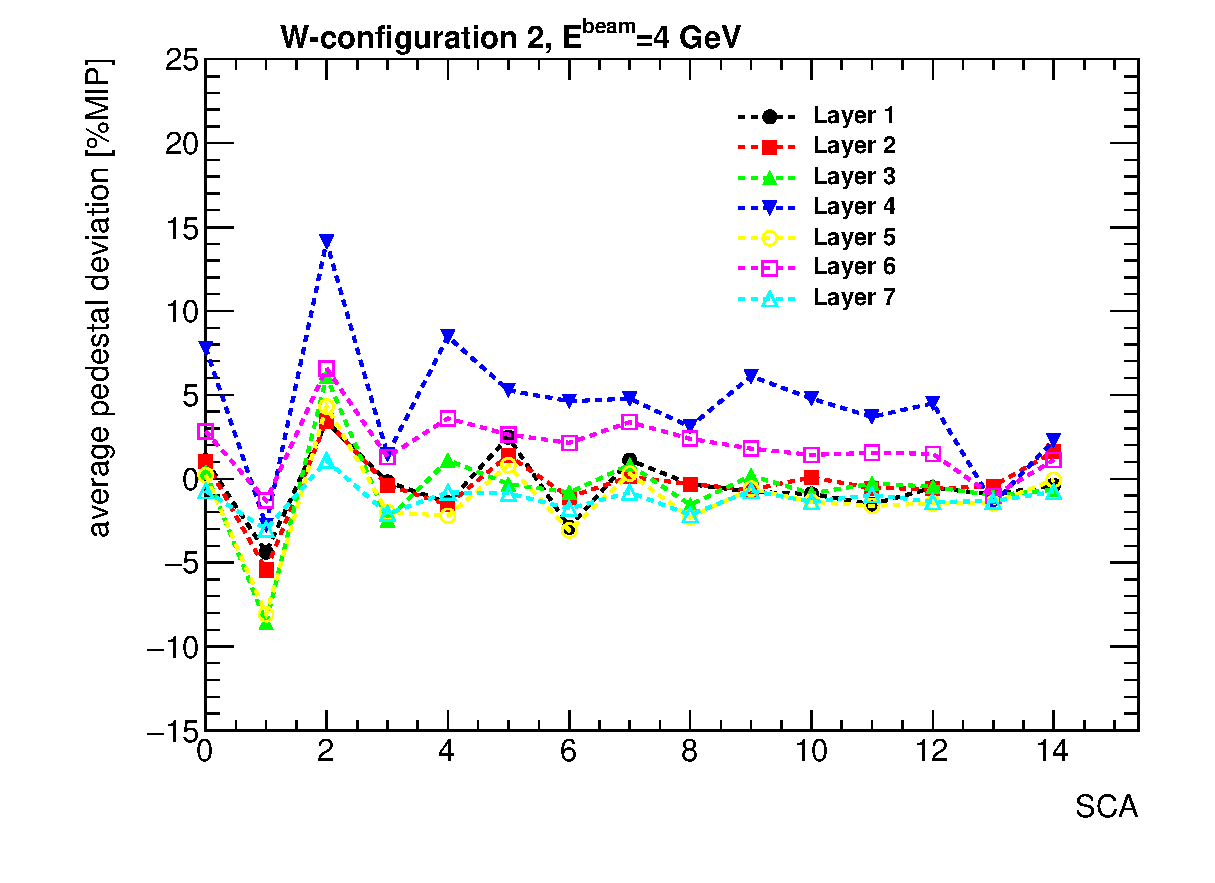
\includegraphics[width=2.8in]{../figs/pedestal/pedestal_deviation_4GeV.eps} \\
    \end{tabular}
    \caption{Average value over all channels in ASIC 12 of the pedestals position for each SCA in electromagnetic shower events.}
\label{pedestal_shower_2}
\end{figure}


\section{Summary}
\label{sec:summary}

The R\&D program of the highly granular SiW-ECAL detector is in an exciting phase. 
After the proof of principle of the imaging calorimetry concept using the physics prototype, the 
technological prototype is being constructed and tested. In this document we describe the commissioning and
beam test performance of a prototype built in with the first fully assembled
detector elements, in contrast with previous beam tests. In addition,
with the setup used in this beam test we reached levels of granularity
similar to the targets of the ILD detector for the ILC. This is also the first time
that a SiW-ECAL prototype continuously takes data in a beam test running in power pulsing mode, one of the crucial
features for the detectors for the ILC. Finally, we tested the performance of the detector
modules working for long periods inside magnetic fields.

A very comprehensive and detailed commissioning procedure has been established and optimized
allowing us to identify and isolate the different noise sources that could spoil the data taking.
The beam test has provided a lot of useful data to study 
the performance of the detector and to perform
a channel by channel calibration, showing a good homogeneity with a spread of the 5\% for all channels.
The signal over noise, S/N, of the detector has been evaluated to be $12.9\pm3.4$ for the trigger
decission and $20.4\pm1.5$ for the charge measurement.

\section{Outlook}
\label{sec:outlook}

In parallel to the work described here, several R\&D efforts are being carried.
One of these efforts is directed to the design and test of new ASICs.
In fact, a new generation of SKIROC2, the 2a, has been delivered
and it is being tested in the dedicated testboards and it has been integrated in new ASUs.
In addition, a new generation of the ASIC, SKIROC3, is foreseen for the final detector construction.
In contrast with SKIROC2/2a, the new ASIC will be fully optimized for ILC operation, {\it i.e.} full zero suppression, reduced power consumption etc.

Many efforts are also concentrated in the construction and test of long SLABs
made of several ASUs enchained since we know that the ILD ECAL will host long layers of up to $\sim$2.5m.
This device constitutes a technological challenge in both aspects, the mechanical
(very thin and long structure with fragile sensors in the bottom make complicated the assembly procedure and the handling...)
and the electrical (we need to ensure and control the transmission of signals and high currents along the full device).
For example, interconnections between ASUs and between ASU and interface card are one of
the most involved parts of the assembly
and require close collaboration between mechanical and electronic engineers.
A first long SLAB prototype
of $\sim8$ ASUs has been already tested in beam test also in DESY in 2018.

In parallel, a different proposal for a thiner ASU
design is being investigated. This is motivated by the high density of channels
demanded by the Particle Flow algorithms. 
In this alternative PCB design the ASICs
are directly placed on board of the PCB in dedicated cavities.
The ASICS will be in semiconductor packaging and wire bonded to the PCB. This is the so-called COB (chip-on-board) version of the ASU.
A small sample of FEV11\_COBs (same connexion pattern with the interface card than FEV11)
with a total thickness of 1.2 mm (to be compared with the 2.7 of the LFBGA solution)
has been produced and tested in the laboratory
showing its readiness for tests with particle beams. A sample can be seen in Figure \ref{cob}.
These new boards maximize the density of channels (6000 channels/dm$^{3}$) for the ECAL of the ILD
and will allow to satisfy the baseline requirements of the ECAL for the ILD.

\begin{figure}[!t]
  \centering
    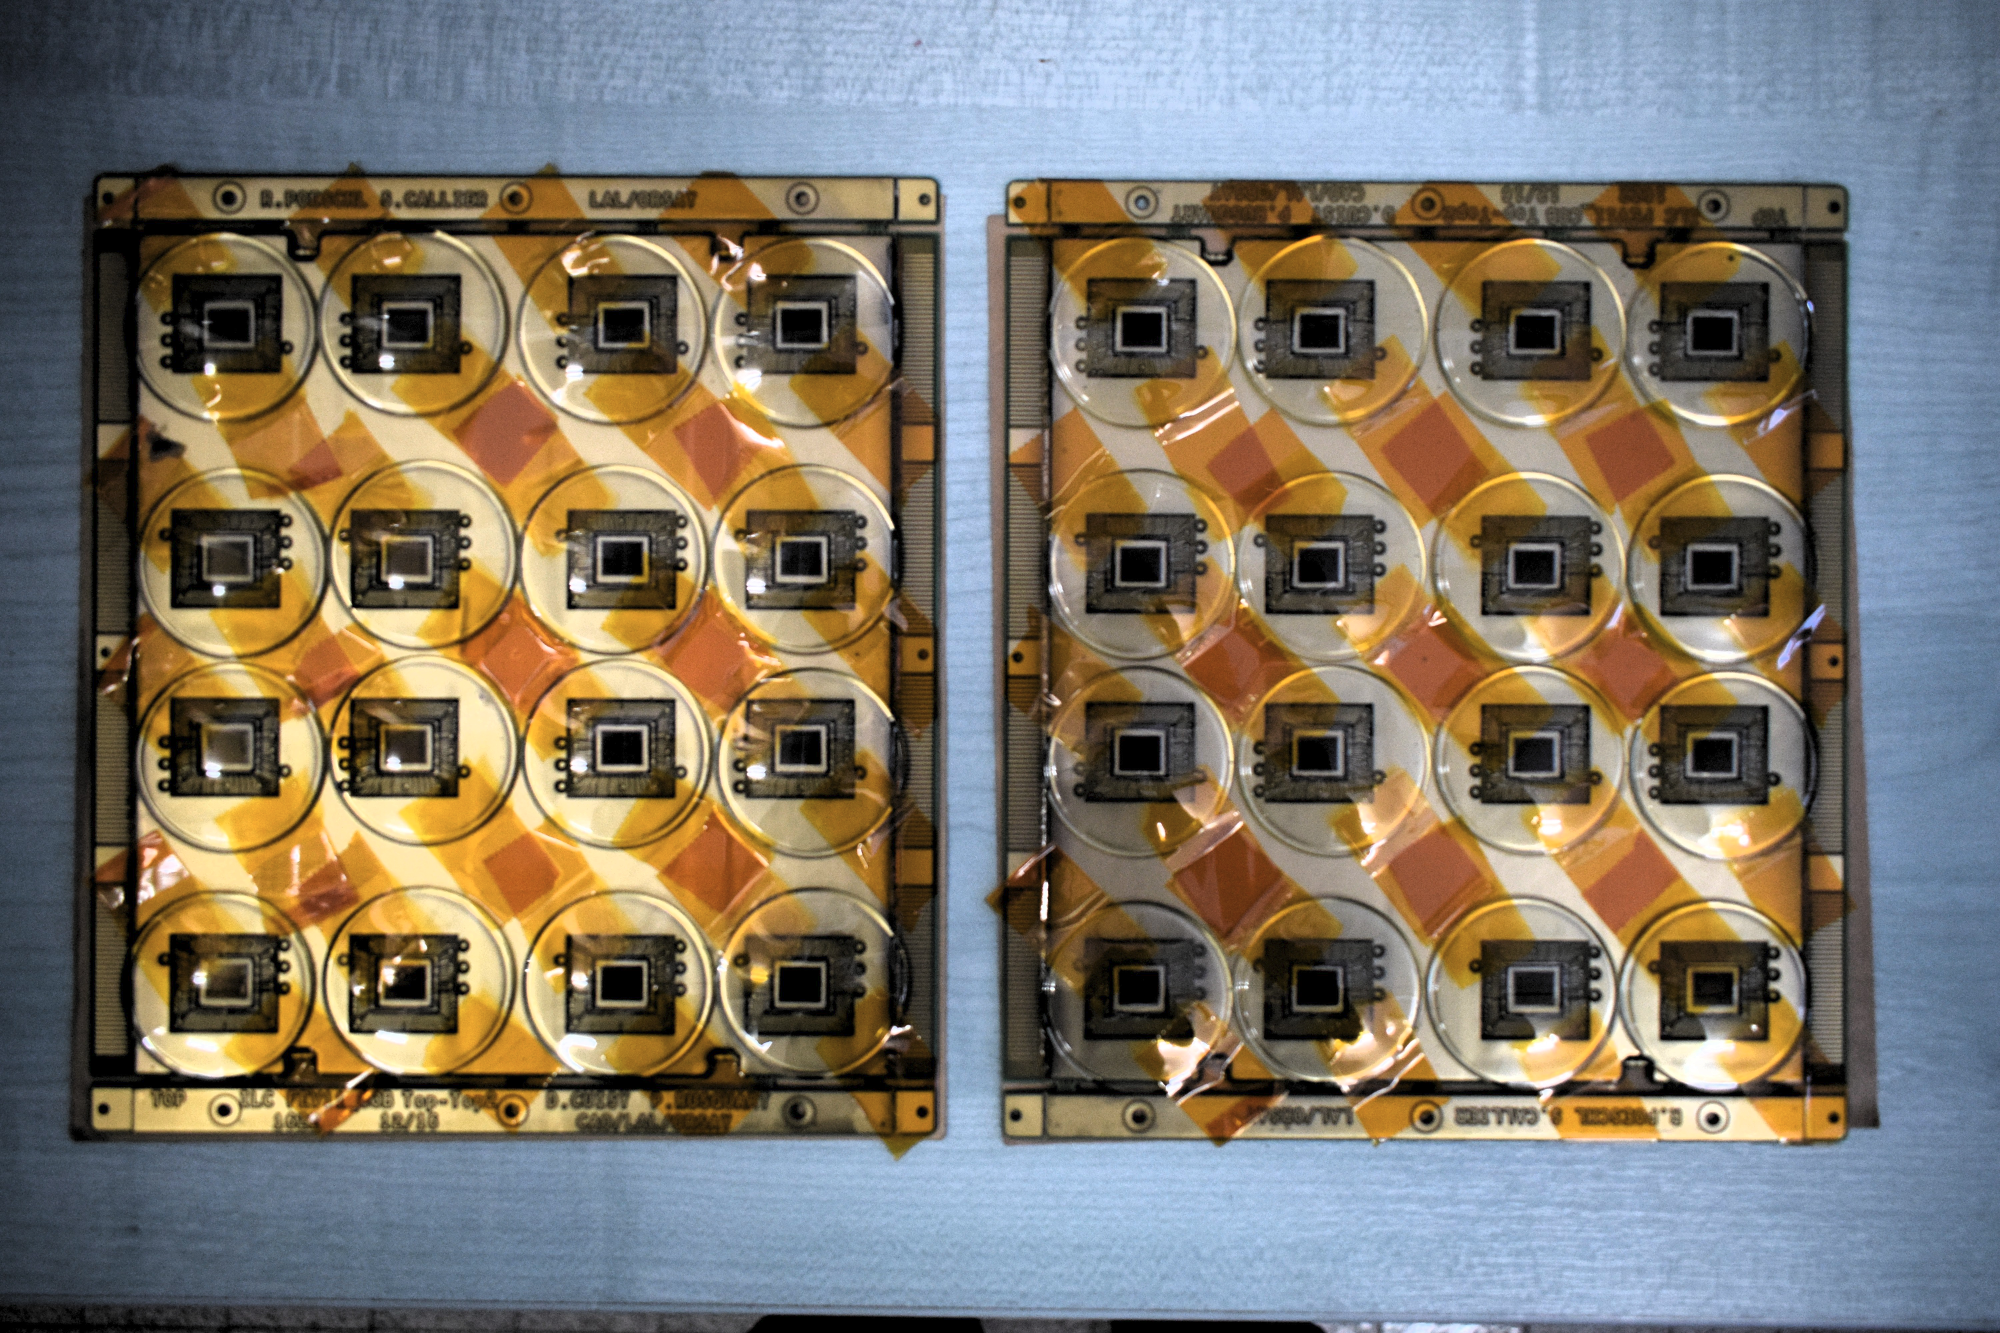
\includegraphics[width=2.8in]{../figs/fev11_cob.png} 
  \caption{Two FEV11\_COB boards with 16 SKIROC2a wire bonded. The ASICs are protected with watch glasses.}
\label{cob}
\end{figure}

Finally, intensive R\&D on the compactification of
the DAQ to meet the tight space requirements for the ILD is being done by the SiW-ECAL collaboration.

It is foreseen that all these developments, with the exception of the SKIROC3, will be tested with particle beams during 2018-2019.


\acknowledgments

This project has received funding from the European Union{\textquotesingle}s Horizon 2020 Research and Innovation program under Grant Agreement no. 654168.
This work was supported by the P2IO LabEx (ANR-10-LABX-0038), excellence project HIGHTEC,
in the framework {\textquotesingle}Investissements d{\textquotesingle}Avenir{\textquotesingle}
(ANR-11-IDEX-0003-01) managed by the French National Research Agency (ANR).
The research leading to these results has received funding from the People Programme (Marie
Curie Actions) of the European Union{\textquotesingle}s Seventh Framework Programme (FP7/2007-2013)
under REA grant agreement, PCOFUND-GA-2013-609102, through the PRESTIGE
programme coordinated by Campus France.
The measurements leading to these results have been performed at the Test Beam Facility at DESY Hamburg (Germany), a member of the Helmholtz Association (HGF).

\appendix
\section{Apendix: Filtering of fake triggers}
\label{sec:retriggers}

Several types of fake signals have been observed in the technollogical prototype since its construction and test. A detailed description of them
can be found in previous articles, as for example, in Ref. \cite{Amjad:2014tha}. All these fake signals are easily identified
and tagged during the data acquisition and removed afterwards from the analysis
not introducing any significance loss of performance as can be seen, for example,
in the hit detection efficiency plots (see Section \ref{sec:calib}).
In the following, we briefly describe the status of the monitoring, debugging and filtering
of such kind of events.

\subsubsection*{Empty triggers}

Empty trigger events are a well known feature of SKIROC2. The SKIROC2 uses
an OR64 signal to mark the the change to a new SCA when a signal over threshold is
detected. The empty triggers appear when during
the acquisition the rising edge of the slow clock falls during the OR64 signal
and therefore the change to a new SCA is validated twice.
This effect creates around 17\% of empty events which are easily filter and removed from the
analysis. The ratio of empty triggers in the new SKIROC2a has been reduced to the $\sim2-3\%$
by reducing the length of the OR64 signal.

\subsubsection*{Plane events and retriggers}

Another well know issue is the appearance of bunches of consecutive fake triggers, called retriggers,
that saturates the DAQ. 
Although the ultimate reason of the appearance of these events remains not clear, it
is suspected that they are related to distortions of the
power supply baselines. We know that the SKIROC2 and 2a preamplifiers are referenced to the analog power supply level,
therefore, any voltage dip can ve seen as signal by the preamplifiers.
Moreover the presence of a high inrush of current
due to many channels triggered at the same time can create these voltage dips
and also produce the so called plane events (most of the channels trigered at once).
In previous studies the ratio of retriggers and plane events
was reduced by improving the power supply stabilization capacitances. %It is important to remark that
%all layers and all ASICs analog and digital levels are powered using the same power supply.
%Moreover, the high voltage power supply for the polarization of the PIN diode is also common for all layers
%and the grounding levels of the low and high voltages supplied are shared within the slab.
%Therefore any noise in
%these power supplies or any overload of an ASIC may participate in the creation of fake signals
%in different ASICs and layers.

Studying the MIP calibration data of this beam test we have noticed that the 
concentration of the retriggers and plane events in
ASICs far from the beam spot is higher than in the ASICs that are reading
out the information of real hits. We have also observed that the concentration of these events
is higher in the nearby of channels that were masked as suspicious of suffering from routing issues.
The ratio these events have been estimated to be of $1-3\%$ in the ASICs where high frequency
interactions are produced ({\it i.e.} using 3 GeV positrons ate 2-3 KHz) and at higher rates even larger than $40\%$ in other 
ASICs far from the beam spot. 
Moreover, it has been noticed a correlation between the time that an ASIC was full and the time of the appearance of some 
retriggers in other areas of the PCB. 
This correlation corresponds to $\sim$1.6 $\mu$s which hints
of a distortion on the analogue power supply when
the signal that informs the DIF that one ASIC memory is full is transmitted through the PCB.

%All this information and dedicated studies in the laboratory will be used for the
%improvement of the power supplying system, the PCB design and for further SKIROC developments 
%with the possible approval the ILC in the scope.

% We suggest to always provide author, title and journal data:
% in short all the informations that clearly identify a document.

\bibliographystyle{JHEP}
\bibliography{../references}

\end{document}
